\chapter{赋范空间与内积空间}
\label{chap:normed-inner-product-spaces}

上一章只使用加法和数乘，能够判断线性表示是否存在、是否唯一，却不能度量两个对象相差多少。本章在线性空间上先加入范数，使大小、误差和收敛有明确含义；再加入内积，讨论角度、正交和子空间中的最佳近似。

赋范空间一节说明有限维范数为何给出相同的收敛结果，以及有限维空间为何完备；对偶范数衡量给定输入误差预算下线性读取的最大变化。内积空间一节利用Gram矩阵、正交分解和标准正交基组织几何计算，再将线性泛函表示与伴随联系起来。本章主要处理有限维空间，一般无限维理论需要另行检查完备性与闭性。

% 第5章第5节：赋范空间（范数与收敛、有限维赋范空间、完备性与Banach空间），只讨论有限维情形。

\section{赋范空间}
\label{sec:ls-normed-spaces}

上一章只用到加法与数乘，回答的都是“能否表示、是否唯一、有几个方向”这类是非与计数问题，还没有“大小”。可是用一个多项式近似一个函数时，要问误差有多大；一列近似越来越好时，要问它们是否趋于某个对象，那个对象是否仍在原来的空间里；上一章的读取也要问，输入不大时读数最多有多大。第~\ref{chap:linear-operations}章用范数度量$\mathbb R^d$中数组的大小，本节把它推广到一般线性空间。

本节回答三个问题：范数怎样给出收敛；有限维空间中，选哪个范数会不会影响收敛与否；收敛序列的极限什么时候一定留在空间中。前两个问题在有限维中有干净的答案：一切范数等价，收敛就是逐坐标收敛。第三个问题引出完备性与Banach空间，它在有限维中自动成立。本节只讨论有限维空间；无限维空间仍可用范数定义收敛，但范数等价与完备性不再自动成立，留到后面的章节。

\subsection{范数、距离与收敛}
\label{sec:ls-normed-space-definition}

\paragraph{范数的定义}
第~\ref{chap:linear-operations}章的$\ell_1$、$\ell_2$、$\ell_\infty$范数各有侧重，所表达的大小应满足同样的几条要求：大小非负，只有零向量大小为零，整体放大$c$倍时大小放大$|c|$倍，两段误差相加时总大小不超过各自大小之和。这些要求只用到加法与数乘，因此可以直接作为一般线性空间上“大小”的要求。
\begin{definition}[赋范空间]
\label{def:ls-normed-space}
\label{def:functional-normed-space}
设$V$是实线性空间。映射$\lVert\cdot\rVert:V\to[0,\infty)$若对任意$\bm x,\bm y\in V$与$c\in\mathbb R$满足
\begin{enumerate}
 \item 正定性：$\lVert\bm x\rVert=0$当且仅当$\bm x=\bm0$；
 \item 齐次性：$\lVert c\bm x\rVert=|c|\,\lVert\bm x\rVert$；
 \item 三角不等式：$\lVert\bm x+\bm y\rVert\leq\lVert\bm x\rVert+\lVert\bm y\rVert$，
\end{enumerate}
就称为$V$上的\term{范数}（norm）；配备范数的线性空间$(V,\lVert\cdot\rVert)$称为\term{赋范空间}（normed space）。
\end{definition}
范数诱导距离$d(\bm x,\bm y)=\lVert\bm x-\bm y\rVert$：它非负，只在$\bm x=\bm y$时为零，对称，并满足$d(\bm x,\bm z)\leq d(\bm x,\bm y)+d(\bm y,\bm z)$。这些性质也是\BookChapterRef{chap:metric-spaces}{第~\ref{chap:metric-spaces}章}度量空间的公理，所以赋范空间是一类特殊的度量空间。它的距离还与线性运算相容：平移不改变距离，缩放把距离按比例缩放。

把三角不等式用于$\bm x=(\bm x-\bm y)+\bm y$，得$\lVert\bm x\rVert-\lVert\bm y\rVert\leq\lVert\bm x-\bm y\rVert$；交换$\bm x,\bm y$的角色，又得$\lVert\bm y\rVert-\lVert\bm x\rVert\leq\lVert\bm x-\bm y\rVert$。两式合起来就是反向三角不等式
\begin{equation}
 \bigl|\lVert\bm x\rVert-\lVert\bm y\rVert\bigr|\leq\lVert\bm x-\bm y\rVert,
 \label{eq:ls-reverse-triangle}
\end{equation}
它说明两个向量相距很近时，长度也相差很少。

\paragraph{坐标范数的公理检验}
\label{sec:ls-norms-distances}
\label{sec:linear-algebra-distance-relations}

第~\ref{sec:ls-vector-operations}节的$p$范数满足非负性、正定性与齐次性，这可以直接从公式读出；需要证明的是三角不等式。$p=1$时，对每个坐标用实数的$|x_j+y_j|\leq|x_j|+|y_j|$再求和即得；$p=\infty$时，同一不等式给出$|x_j+y_j|\leq\lVert\bm x\rVert_\infty+\lVert\bm y\rVert_\infty$，再对$j$取最大值即得。$1<p<\infty$时，先要建立下面的不等式，它用一对互相配合的$p$范数与$q$范数控制两个向量逐项乘积之和。

\paragraph{Hölder不等式}
先估计两个向量逐坐标相乘后的总和。下面的共轭指数条件使两个范数能够配合使用。
\begin{theorem}[有限维Hölder不等式]
\label{thm:linear-algebra-holder}
设$1\leq p,q\leq\infty$且$1/p+1/q=1$（约定$1/\infty=0$），则$|\bm x^\top\bm y|\leq\lVert\bm x\rVert_p\lVert\bm y\rVert_q$。
\end{theorem}
\begin{proof}
先设$1<p,q<\infty$，分三步证明。

第一步，证明Young不等式：对$u,v\geq0$，
\[
 uv\leq\frac{u^p}{p}+\frac{v^q}{q}.
\]
$u=0$时左侧为零，不等式成立。$u>0$时令$t=v/u^{p-1}\geq0$。由$1/p+1/q=1$得$(p-1)q=p$，于是$v^q=t^qu^p$、$uv=tu^p$，不等式化为
\[
 u^p\Bigl(\frac1p+\frac{t^q}{q}-t\Bigr)\geq0.
\]
函数$f(t)=1/p+t^q/q-t$的导数$t^{q-1}-1$在$0<t<1$时为负、在$t>1$时为正，所以$f$在$t\geq0$上的最小值是$f(1)=1/p+1/q-1=0$，不等式成立。

第二步，在单位尺度下求和。若$\bm x$或$\bm y$为零向量，结论两侧都为零。否则令$u_j=|x_j|/\lVert\bm x\rVert_p$、$v_j=|y_j|/\lVert\bm y\rVert_q$，则$\sum_ju_j^p=\sum_jv_j^q=1$。对每个$j$用Young不等式再求和，
\[
 \sum_ju_jv_j\leq\frac1p\sum_ju_j^p+\frac1q\sum_jv_j^q=\frac1p+\frac1q=1.
\]

第三步，恢复尺度。上式两边乘以$\lVert\bm x\rVert_p\lVert\bm y\rVert_q$，再用$|\bm x^\top\bm y|\leq\sum_j|x_j||y_j|$，即得
\[
 |\bm x^\top\bm y|\leq\sum_j|x_j||y_j|\leq\lVert\bm x\rVert_p\lVert\bm y\rVert_q.
\]

端点情形直接估计。$p=1$、$q=\infty$时，
\[
 \sum_j|x_j||y_j|\leq\Bigl(\max_j|y_j|\Bigr)\sum_j|x_j|=\lVert\bm x\rVert_1\lVert\bm y\rVert_\infty;
\]
$p=\infty$、$q=1$时交换两个向量的角色。
\end{proof}
$p=q=2$时，它给出$|\bm x^\top\bm y|\leq\lVert\bm x\rVert_2\lVert\bm y\rVert_2$。第~\ref{sec:ls-inner-product-definition}节将只用内积公理，对任一内积证明同样形式的不等式，即Cauchy--Schwarz不等式。

\paragraph{Minkowski不等式}
Hölder不等式控制逐项乘积的和。将它用于向量和的各个坐标，就能证明$p$范数满足三角不等式。
\begin{theorem}[有限维Minkowski不等式]
\label{thm:linear-algebra-minkowski}
设$\bm x,\bm y\in\mathbb R^d$，$1\leq p\leq\infty$，则
\[
 \lVert\bm x+\bm y\rVert_p\leq\lVert\bm x\rVert_p+\lVert\bm y\rVert_p.
\]
\end{theorem}
\begin{proof}
先处理两个端点。$p=1$时，对每个坐标使用实数的三角不等式，再求和，得到
\[
 \sum_j|x_j+y_j|\leq\sum_j|x_j|+\sum_j|y_j|.
\]
$p=\infty$时，对每个$j$都有
\[
 |x_j+y_j|\leq\lVert\bm x\rVert_\infty+\lVert\bm y\rVert_\infty.
\]
左侧对$j$取最大值，就得到所需结论。

下面设$1<p<\infty$。若$\bm x+\bm y=\bm0$，左侧为零，结论成立；以下只需考虑和向量非零的情形。取$q=p/(p-1)$，则$1/p+1/q=1$。对每个坐标有
\[
 \begin{aligned}
 |x_j+y_j|^p
 &=|x_j+y_j|^{p-1}|x_j+y_j|\\
 &\leq |x_j+y_j|^{p-1}(|x_j|+|y_j|).
 \end{aligned}
\]
令$s_j=|x_j+y_j|^{p-1}$，把这些数排成向量$\bm s$。由于$(p-1)q=p$，它的$q$范数为
\[
 \begin{aligned}
 \lVert\bm s\rVert_q
 &=\Bigl(\sum_j|x_j+y_j|^p\Bigr)^{1/q}\\
 &=\lVert\bm x+\bm y\rVert_p^{p-1}.
 \end{aligned}
\]
把逐坐标的不等式求和，并对包含$|x_j|$和$|y_j|$的两部分分别使用Hölder不等式，得到
\[
 \begin{aligned}
 \lVert\bm x+\bm y\rVert_p^p
 &\leq\sum_js_j|x_j|+\sum_js_j|y_j|\\
 &\leq\lVert\bm s\rVert_q
       \bigl(\lVert\bm x\rVert_p+\lVert\bm y\rVert_p\bigr)\\
 &=\lVert\bm x+\bm y\rVert_p^{p-1}
       \bigl(\lVert\bm x\rVert_p+\lVert\bm y\rVert_p\bigr).
 \end{aligned}
\]
两边除以正数$\lVert\bm x+\bm y\rVert_p^{p-1}$，即得结论。
\end{proof}
结合前面已经核对的非负性、正定性与齐次性，每个$p$范数都满足范数的四条要求。特别地，欧氏长度满足三角不等式。

\paragraph{常用范数之间的比较}
对$\bm x\in\mathbb R^d$，
\[
 \begin{gathered}
 \lVert\bm x\rVert_\infty\leq\lVert\bm x\rVert_2\leq\sqrt d\,\lVert\bm x\rVert_\infty,
 \\
 \lVert\bm x\rVert_2\leq\lVert\bm x\rVert_1\leq\sqrt d\,\lVert\bm x\rVert_2.
 \end{gathered}
\]
左端两式的依据是：平方和不小于其中最大的一项，所以$\lVert\bm x\rVert_\infty^2\leq\lVert\bm x\rVert_2^2$；展开$(\sum_j|x_j|)^2$时交叉项非负，所以$\lVert\bm x\rVert_1^2\geq\sum_jx_j^2=\lVert\bm x\rVert_2^2$。右端两式的依据是：$\sum_jx_j^2\leq d\max_jx_j^2$给出$\lVert\bm x\rVert_2\leq\sqrt d\,\lVert\bm x\rVert_\infty$；把$\sum_j|x_j|$看作$(|x_1|,\ldots,|x_d|)^\top$与全$1$向量的内积，用$p=q=2$的Hölder不等式，得到$\lVert\bm x\rVert_1\leq\sqrt d\,\lVert\bm x\rVert_2$。

下面在示例~\ref{ex:ls-p-norms}的向量上核对这四个不等式。
\begin{example}[范数比较的数值核对]
\label{ex:ls-norm-comparison-check}
给定：$d=2$，$\bm x=(3,-4)^\top$；由示例~\ref{ex:ls-p-norms}，$\lVert\bm x\rVert_1=7$，$\lVert\bm x\rVert_2=5$，$\lVert\bm x\rVert_\infty=4$。
验证：
\[
 \begin{gathered}
 4\leq5\leq4\sqrt2\approx5.66,\\
 5\leq7\leq5\sqrt2\approx7.07.
 \end{gathered}
\]
结论：四个不等式都成立。右端的$\sqrt2$都不能换成$1$：$\lVert\bm x\rVert_2=5$大于$\lVert\bm x\rVert_\infty=4$，$\lVert\bm x\rVert_1=7$也大于$\lVert\bm x\rVert_2=5$。
\end{example}
右端的常数随维数增大，而且一般不能改小：全$1$向量$\bm 1\in\mathbb R^d$满足$\lVert\bm 1\rVert_\infty=1$、$\lVert\bm 1\rVert_2=\sqrt d$、$\lVert\bm 1\rVert_1=d$，两个右端不等式都取等号。所以维数较大时，$\sqrt d$不能在误差预算中忽略。


有时只关心向量的一部分信息，这时允许非零向量的大小为零，但保留齐次性与三角不等式。这样的尺度称为\term{半范数}（seminorm）。它给出的“距离”可能把不同的点判为距离为零，下面的例子说明这一点。
\begin{example}[只看第一个坐标的半范数]
\label{ex:ls-seminorm-first-coordinate}
给定：$\mathbb R^2$上的函数$p(\bm x)=|x_1|$。
验证：$p(\bm x)\geq0$；$p(c\bm x)=|cx_1|=|c|\,p(\bm x)$；$p(\bm x+\bm y)=|x_1+y_1|\leq|x_1|+|y_1|=p(\bm x)+p(\bm y)$。所以$p$满足非负性、齐次性与三角不等式。但非零向量$(0,1)^\top$满足$p\bigl((0,1)^\top\bigr)=0$，正定性不成立。
结论：$p$是半范数而不是范数。它判定$(0,0)^\top$与$(0,1)^\top$的距离为$p\bigl((0,-1)^\top\bigr)=0$，完全忽略了第二个坐标上的差别。
\end{example}
使用半范数之前，须先说明哪些差别被有意忽略。

\paragraph{例子}
$\mathbb R^d$上的$p$范数、同形矩阵上的Frobenius范数与诱导矩阵范数都是范数，其中$p$范数已在上面验证，Frobenius范数是将矩阵元素排成向量后的$2$范数；诱导矩阵范数将在第~\ref{sec:ls-matrix-norms}节定义并验证。一般空间上，最直接的办法是借坐标：若$\lVert\cdot\rVert_\star$是$\mathbb R^d$上的范数，$\mathcal B$是$V$的基，则$\lVert\bm v\rVert=\lVert[\bm v]_{\mathcal B}\rVert_\star$是$V$上的范数，因为坐标映射是保持线性组合的双射。也可以不经过坐标，直接用对象本身的性质规定范数。下面在$P_k$上各举一例。
\begin{example}[多项式空间上的两个范数]
\label{ex:ls-polynomial-norms}
给定：$P_k$上的两个规则：对$p=a_0+a_1t+\cdots+a_kt^k$，
\[
\begin{gathered}
p\mapsto\max_{0\leq j\leq k}|a_j|\\
p\mapsto\lVert p\rVert_\infty=\max_{t\in[0,1]}|p(t)| .
\end{gathered}
\]

验证：第一个规则是坐标$(a_0,\ldots,a_k)$在基$(1,t,\ldots,t^k)$下的$\ell_\infty$范数，按上面的借坐标方法是范数。对第二个规则，齐次性逐点成立；三角不等式来自$|p(t)+q(t)|\leq|p(t)|+|q(t)|\leq\lVert p\rVert_\infty+\lVert q\rVert_\infty$对每个$t$成立，再对$t$取最大值；正定性来自次数不超过$k$的非零多项式至多有$k$个根，不能在整个区间$[0,1]$上为零。

结论：二者都是$P_k$上的范数，前者经过坐标，后者直接用函数值。
\end{example}

\paragraph{收敛}
有了距离，就可以说一列向量趋于某个向量。在赋范空间中，若实数列$\lVert\bm x_n-\bm x\rVert\to0$，就说$\bm x_n$按该范数\emph{收敛}到$\bm x$，记为$\bm x_n\to\bm x$。极限若存在则唯一：若$\bm x_n\to\bm x$且$\bm x_n\to\bm y$，则$\lVert\bm x-\bm y\rVert\leq\lVert\bm x-\bm x_n\rVert+\lVert\bm x_n-\bm y\rVert\to0$。由式~\eqref{eq:ls-reverse-triangle}，$\bm x_n\to\bm x$时还有$\lVert\bm x_n\rVert\to\lVert\bm x\rVert$。

收敛的定义依赖所选的范数：不同范数给出的误差读数不同，同一个序列会不会在一种范数下收敛、在另一种范数下不收敛？下一小节说明，有限维空间中不会出现这种情形。

\subsection{有限维范数等价}
\label{sec:ls-finite-dimensional-sequences}
\label{sec:linear-algebra-sequence-convergence}
\label{sec:ls-error-scale-comparison}

讨论向量序列的收敛，先要选一个范数测量误差。$\ell_1$、$\ell_2$、$\ell_\infty$或某个加权范数给出的误差读数各不相同。本小节证明，在有限维空间中任意两个范数最多相差常数倍，因而收敛与否、极限是什么都与范数无关；证明要把第~\ref{chap:limits-continuity}章有界实数列的Bolzano--Weierstrass定理逐坐标用于向量序列。由此还得到线性映射的连续性、子空间的闭性与最近点的存在。

\paragraph{闭集与有界集}
在赋范空间中，若存在$R$使$\lVert\bm x\rVert\leq R$对集合$K$中的一切$\bm x$成立，就称$K$\emph{有界}；若$K$中任何收敛序列的极限仍属于$K$，就称$K$\emph{闭}。在实轴上，这一闭性与第~\ref{chap:limits-continuity}章用补集定义的闭集一致（引理~\ref{lem:analysis-closed-sequence-criterion}）；一般度量空间中的开闭集在\BookChapterRef{chap:metric-spaces}{第~\ref{chap:metric-spaces}章}讨论。

闭球$\{\bm x:\lVert\bm x\rVert\leq r\}$是闭集：若$\lVert\bm x_n\rVert\leq r$且$\bm x_n\to\bm x$，则$\lVert\bm x\rVert=\lim_n\lVert\bm x_n\rVert\leq r$。同理，单位球面$\{\bm x:\lVert\bm x\rVert=1\}$是闭有界集。若$K\subseteq V$上的函数$f$满足：只要$K$中的$\bm x_n\to\bm x\in K$，就有$f(\bm x_n)\to f(\bm x)$，就称$f$在$K$上连续。由式~\eqref{eq:ls-reverse-triangle}，范数本身是连续函数。

\paragraph{范数等价}
现在比较同一个有限维空间上的两个范数。
\begin{theorem}[有限维范数等价]
\label{thm:ls-norm-equivalence}
有限维实线性空间上任意两个范数$p,q$都等价：存在常数$c,C>0$，使$c\,q(\bm x)\leq p(\bm x)\leq C\,q(\bm x)$对所有$\bm x$成立。
\end{theorem}
\begin{proof}
思路是把每个范数都与一个固定的参照范数比较。固定基$(\bm b_1,\ldots,\bm b_d)$，把$\bm x=\sum_jx_j\bm b_j$等同于坐标向量$(x_1,\ldots,x_d)$，取坐标最大范数$\lVert\bm x\rVert_c=\max_j|x_j|$作参照。按它收敛就是逐坐标收敛：$\lVert\bm x_n-\bm x\rVert_c\to0$当且仅当每个坐标$x_{n,j}\to x_j$，因为最大值趋于零当且仅当有限个坐标差都趋于零。

上界。对任意范数$p$，由三角不等式与齐次性，
\[
 \begin{gathered}
p(\bm x)=p\Bigl(\sum_jx_j\bm b_j\Bigr)\leq\sum_j|x_j|\,p(\bm b_j)\leq C_p\lVert\bm x\rVert_c\\
C_p=\sum_jp(\bm b_j).
 \end{gathered}
\]

下界。由反向三角不等式，$|p(\bm x)-p(\bm y)|\leq p(\bm x-\bm y)\leq C_p\lVert\bm x-\bm y\rVert_c$，所以只要$\lVert\bm x_n-\bm x\rVert_c\to0$，就有$p(\bm x_n)\to p(\bm x)$。考虑坐标单位球面$S=\{\bm x:\lVert\bm x\rVert_c=1\}$，记$m_p=\inf_{\bm x\in S}p(\bm x)\geq0$，对每个$n$取$\bm x_n\in S$使$p(\bm x_n)<m_p+1/n$。这列向量的每个坐标都满足$|x_{n,j}|\leq1$，是有界实数列。由Bolzano--Weierstrass定理~\ref{thm:analysis-bounded-subsequence}，先在第一坐标上抽出收敛子列，再在这个子列中按第二坐标继续抽取，如此重复$d$次，最后得到的子列$\bm x_{n_k}$在每个坐标上都收敛。记各坐标的极限组成的向量为$\bm x^\star$，则$\lVert\bm x_{n_k}-\bm x^\star\rVert_c\to0$；由$\lVert\cdot\rVert_c$的反向三角不等式，$\lVert\bm x^\star\rVert_c=\lim_k\lVert\bm x_{n_k}\rVert_c=1$，即$\bm x^\star\in S$。再由上面$p$的连续性，\phantomsection\label{thm:ls-extreme-value}$p(\bm x^\star)=\lim_kp(\bm x_{n_k})=m_p$，即$p$在$S$上取到最小值$m_p$。由$\lVert\bm x^\star\rVert_c=1$知$\bm x^\star\neq\bm0$，范数的正定性保证$m_p=p(\bm x^\star)>0$。对任意$\bm x\neq\bm0$，$\bm x/\lVert\bm x\rVert_c$在$S$上，由齐次性得$p(\bm x)\geq m_p\lVert\bm x\rVert_c$。合起来，
\begin{equation}
 m_p\lVert\bm x\rVert_c\leq p(\bm x)\leq C_p\lVert\bm x\rVert_c.
 \label{eq:linear-algebra-finite-norm-equivalence}
\end{equation}

最后比较$p$与$q$：$p\leq C_p\lVert\cdot\rVert_c\leq(C_p/m_q)\,q$，交换$p,q$的角色得反向不等式。
\end{proof}
定理中的常数依赖维数与所选范数。看$\ell_1$与$\ell_\infty$这一对。
\begin{example}[$\ell_1$与$\ell_\infty$范数的等价常数]
\label{ex:ls-l1-linf-constants}
给定：$\mathbb R^d$上的$\lVert\bm x\rVert_1=\sum_j|x_j|$与$\lVert\bm x\rVert_\infty=\max_j|x_j|$。

验证：$d$个非负数$|x_1|,\ldots,|x_d|$之和不小于其中最大的一个，又不超过最大者的$d$倍，所以
\[
 \lVert\bm x\rVert_\infty\leq\lVert\bm x\rVert_1\leq d\lVert\bm x\rVert_\infty .
\]
取$\bm x=\bm e_1$，两个范数都为$1$，左边取等号；取$\bm x=(1,\ldots,1)^\top$，$\lVert\bm x\rVert_1=d$、$\lVert\bm x\rVert_\infty=1$，右边取等号。

结论：常数$1$与$d$都不能改进；维数越大，同一误差在两种范数下的读数可以相差越多。
\end{example}
证明中真正用到有限维的是下界：坐标只有有限个，逐坐标抽取$d$次才得到在每个坐标上都收敛的子列，从而在单位球面上取到正的最小值。

\paragraph{收敛与连续性}
由范数等价，$\lVert\bm x_n-\bm x\rVert\to0$当且仅当$\lVert\bm x_n-\bm x\rVert_c\to0$，即每个坐标$x_{n,j}\to x_j$。因此在有限维空间中，序列是否收敛、收敛到哪里，都与所选范数和基无关，后文可以按论证方便选用范数。矩阵序列看作$\mathbb R^{m\times n}$中的向量，结论相同：$\bm A_k\to\bm A$在任意矩阵范数下都等价于逐元素收敛。

闭集与有界集同样与范数无关：两个范数只差常数倍，一个范数下有界的集合在另一个范数下也有界，收敛序列也完全相同。于是下界证明中的逐坐标抽取对任何范数都适用：有界序列的坐标有界，可以抽出收敛子列；若序列取自闭集，极限仍在集合内。

由此得到闭有界集上连续函数的最值。

设$f$是非空闭有界集$K$上的连续函数，$m=\inf_{K}f$。取$K$中的序列$\bm x_n$，使$f(\bm x_n)\to m$（若$m=-\infty$，则使$f(\bm x_n)\to-\infty$），从中抽出收敛子列$\bm x_{n_k}\to\bm x^\star$；由闭性，$\bm x^\star\in K$。由连续性，$f(\bm x_{n_k})\to f(\bm x^\star)$。若$m=-\infty$，这个有限极限与$f(\bm x_{n_k})\to-\infty$矛盾，所以$m$有限；于是$f(\bm x^\star)=\lim_kf(\bm x_{n_k})=m$，即下确界可以取到。上确界同理。下面几处“可以达到”都由这一论证得到。

线性映射也自动连续。

设$T:V\to W$是有限维赋范空间之间的线性映射，固定$V$的基并沿用证明中的记号。由三角不等式与齐次性，
\[
\begin{gathered}
\lVert T\bm x\rVert_W\leq\sum_j|x_j|\,\lVert T\bm b_j\rVert_W\leq C\lVert\bm x\rVert_c\leq\frac C{m_V}\lVert\bm x\rVert_V\\
C=\sum_j\lVert T\bm b_j\rVert_W,
\end{gathered}
\]
其中$m_V>0$是式~\eqref{eq:linear-algebra-finite-norm-equivalence}中$\lVert\cdot\rVert_V$的下界常数。于是$\lVert T\bm x_n-T\bm x\rVert_W\leq(C/m_V)\lVert\bm x_n-\bm x\rVert_V$，$T$连续。

上式还说明比值$\lVert T\bm x\rVert_W/\lVert\bm x\rVert_V$有界。由上面的最值论证，连续函数$\bm x\mapsto\lVert T\bm x\rVert_W$在闭且有界的单位球面上取到最大值，所以后面定义的诱导矩阵范数具有有限且可达到的上确界。取$W=\mathbb R$，就回答了上一章留下的问题：线性泛函$\varphi$的大小可以定义为
\[
 \lVert\varphi\rVert_*=\sup_{\lVert\bm x\rVert\leq1}|\varphi(\bm x)|,
\]
它有限并且取到，是对偶空间$V^*$上的范数；在$\mathbb R^d$上，$\varphi(\bm x)=\bm z^\top\bm x$时它正是第~\ref{sec:ls-dual-norms}节的对偶范数$\lVert\bm z\rVert_*$。

\subsection{有限维完备性与子空间}
\phantomsection

点到子空间的距离为零，是否意味着点就在子空间里？这取决于子空间是否闭。
\begin{theorem}[有限维子空间闭性]
\label{thm:ls-subspace-closed}
有限维赋范空间的每个线性子空间$U$都是闭集：若$\bm x_n\in U$且$\bm x_n\to\bm x$，则$\bm x\in U$。
\end{theorem}
\begin{proof}
把$U$的基扩充为整个空间的基，则$\bm x_n$在补充方向上的坐标恒为零。收敛等价于逐坐标收敛，所以$\bm x$在补充方向上的坐标是零序列的极限，仍为零，于是$\bm x\in U$。
\end{proof}
记点到子空间的距离为$d(\bm x,U)=\inf_{\bm u\in U}\lVert\bm x-\bm u\rVert$。若$d(\bm x,U)=0$，可在$U$中取$\bm u_n$使$\lVert\bm x-\bm u_n\rVert\to0$，由闭性$\bm x\in U$；反之显然。所以$d(\bm x,U)=0$当且仅当$\bm x\in U$。

\paragraph{完备性}
\label{sec:ls-banach-spaces}

收敛的定义要求事先知道极限$\bm x$。迭代算法、级数截断等过程却常常只给出一列越来越接近彼此的近似，极限是什么、在不在空间里，事先并不知道。第~\ref{chap:limits-continuity}章对实数列用柯西条件回答了这个问题；本小节把它搬到赋范空间，并说明它在有限维中总是可用。

\paragraph{柯西列与完备性}
赋范空间中的序列$\bm x_n$若满足：对任意$\varepsilon>0$，存在$N$使$m,n>N$时$\lVert\bm x_m-\bm x_n\rVert<\varepsilon$，就称为柯西列。收敛序列都是柯西列：若$\bm x_n\to\bm x$，则$\lVert\bm x_m-\bm x_n\rVert\leq\lVert\bm x_m-\bm x\rVert+\lVert\bm x-\bm x_n\rVert$。反过来，柯西列只检查序列内部，不引用任何候选极限；它是否收敛，取决于空间里有没有那个极限。若赋范空间中每个柯西列都收敛到空间中的某个元素，就称该空间\term{完备}（complete）；完备的赋范空间称为\term{Banach空间}（Banach space，也译作巴拿赫空间）。实数在通常距离下完备，这正是第~\ref{chap:limits-continuity}章的柯西收敛准则。

\begin{theorem}[有限维赋范空间的完备性]
\label{thm:ls-finite-dimensional-complete}
有限维赋范空间在任意范数下都完备，因而是Banach空间；它的每个子空间也完备。
\end{theorem}
\begin{proof}
设$\bm x^{(m)}$是柯西列。由范数等价，$\lVert\bm x^{(m)}-\bm x^{(n)}\rVert_c\leq\lVert\bm x^{(m)}-\bm x^{(n)}\rVert/m_0$，其中$m_0>0$是式~\eqref{eq:linear-algebra-finite-norm-equivalence}中的下界常数，所以每个坐标都是实柯西数列，由实数的完备性各有极限$x_j$。令$\bm x=\sum_jx_j\bm b_j$，有限个坐标的差同时趋于零，所以$\lVert\bm x^{(m)}-\bm x\rVert_c\to0$，再由范数等价得$\bm x^{(m)}\to\bm x$。子空间本身也是有限维赋范空间，同样完备；这也与定理~\ref{thm:ls-subspace-closed}一致：子空间中的柯西列在大空间中有极限，而极限留在闭的子空间里。
\end{proof}
证明的关键是有限维：坐标只有有限个，“每个坐标都收敛”就推出“最大坐标差趋于零”。坐标有无穷多个时这一步会失败：无限维赋范空间未必完备，是否完备取决于空间与范数的搭配。一般度量空间的完备性见\BookChapterRef{chap:metric-spaces}{第~\ref{chap:metric-spaces}章}，函数空间的完备性见\BookChapterRef{chap:functional-analysis-and-approximation}{第~\ref{chap:functional-analysis-and-approximation}章}。

完备性的用处在于，只要能证明近似序列是柯西列，就能断定极限存在并且仍在空间中，而不必事先找出极限。有限维中这一点由定理~\ref{thm:ls-finite-dimensional-complete}自动保证，所以第~\ref{chap:linear-analysis}章与第~\ref{chap:linear-equations-and-optimization}章讨论矩阵幂、迭代与级数的收敛时，只需估计误差，不必担心极限落到空间之外。范数等价只给出夹逼常数，用于在不同范数之间互换收敛结论，并不提供衰减速度：同一个收敛序列在一种范数下单调下降，在另一种范数下可能先上升，速度要在选定的范数中由递推结构给出。

\subsection{矩阵范数}
\label{sec:ls-matrix-norms}
\label{sec:ch06-map-comparison}
\label{sec:matrix-analysis-norms-effective-rank}

运算章用Frobenius范数衡量矩阵元素的总体大小。另一种口径把矩阵当作计算$\bm x\mapsto\bm A\bm x$，问它最多把输入放大多少倍；误差分析更关心这一种。
\begin{definition}[由向量范数诱导的矩阵范数]
\label{def:matrix-analysis-induced-norm}
给定输入范数$\lVert\cdot\rVert_\alpha$和输出范数$\lVert\cdot\rVert_\beta$，\term{诱导矩阵范数}（induced matrix norm）为
\[
 \lVert\bm A\rVert_{\alpha\to\beta}
 =\sup_{\bm x\neq0}\frac{\lVert\bm A\bm x\rVert_\beta}{\lVert\bm x\rVert_\alpha}.
\]
两端采用同一类$p$范数时简写为$\lVert\bm A\rVert_p$。
\end{definition}
由定义，对每个$\bm x$都有$\lVert\bm A\bm x\rVert_\beta\leq\lVert\bm A\rVert_{\alpha\to\beta}\lVert\bm x\rVert_\alpha$，而且诱导范数是使这一不等式对全部$\bm x$成立的最小常数。

三种常用的诱导范数中，前两种有直接的算法：
\[
 \begin{gathered}
 \lVert\bm A\rVert_1=\max_j\sum_i|a_{i,j}|,\\
 \lVert\bm A\rVert_\infty=\max_i\sum_j|a_{i,j}|,
 \end{gathered}
\]
即最大绝对列和与最大绝对行和，推导放在本小节后面的矩阵范数性质中。第三种是诱导$2$范数，也称\term{谱范数}（spectral norm），$\lVert\bm A\rVert_2=\sup_{\lVert\bm x\rVert_2=1}\lVert\bm A\bm x\rVert_2$，它的计算要用到第~\ref{sec:ls-svd}节的奇异值。

下面在同一个矩阵上比较两种诱导范数与Frobenius范数。
\begin{example}[同一矩阵在不同口径下的大小]
\label{ex:ls-matrix-norms-shear}
给定：$\bm A=\left[\begin{smallmatrix}1&1\\0&1\end{smallmatrix}\right]$。
计算：两列的绝对值之和分别为$1+0=1$与$1+1=2$，两行的绝对值之和分别为$1+1=2$与$0+1=1$，全部元素的平方和为$1+1+0+1=3$。所以
\[
 \begin{gathered}
 \lVert\bm A\rVert_1=\max\{1,2\}=2,\\
 \lVert\bm A\rVert_\infty=\max\{2,1\}=2,\\
 \lVert\bm A\rVert_{\mathrm F}=\sqrt3.
 \end{gathered}
\]
结论：不同口径给出的数值不必相同。
\end{example}
图~\ref{fig:ls-induced-norm-action}画出谱范数的几何意义：单位圆被$\bm A$拉成椭圆，椭圆最长半轴的长度就是最大放大倍数。
\begin{figure*}[htbp]
  \centering
  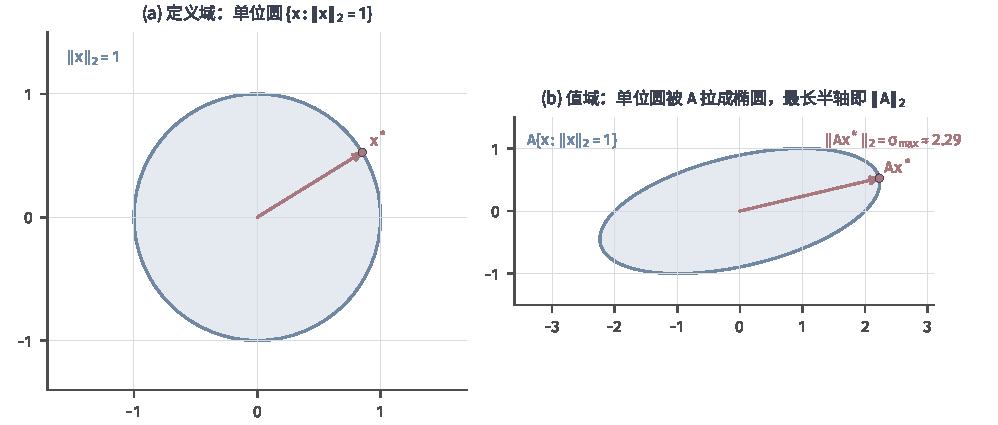
\includegraphics[width=169mm]{figures/00-shared/mathematical-preliminaries-upper/02-linear-spaces/matplotlib/ls-induced-norm-action/ls-induced-norm-action.pdf}
  \caption{诱导矩阵范数衡量最坏放大倍数。左：单位圆$\lVert\bm x\rVert_2=1$；中：同一线性作用$\bm A$把单位圆映成椭圆；右：椭圆上最长的轴给出$\lVert\bm A\rVert_2=\max_{\lVert\bm x\rVert_2=1}\lVert\bm A\bm x\rVert_2$，箭头指示最大放大方向。数值由$\bm A$的教学构造直接得到，是解析例。}
  \label{fig:ls-induced-norm-action}
\end{figure*}


\subsubsection{矩阵范数的性质}

\paragraph{列和与行和公式}
\[
 \begin{gathered}
 \lVert\bm A\rVert_1=\max_j\sum_i|a_{i,j}|,\\
 \lVert\bm A\rVert_\infty=\max_i\sum_j|a_{i,j}|.
 \end{gathered}
\]
第一式按列算：
\[
 \lVert\bm A\bm x\rVert_1=\Bigl\lVert\sum_jx_j\bm A_{:,j}\Bigr\rVert_1\leq\sum_j|x_j|\,\lVert\bm A_{:,j}\rVert_1\leq\Bigl(\max_j\lVert\bm A_{:,j}\rVert_1\Bigr)\lVert\bm x\rVert_1,
\]
而取$\bm x$为最大绝对列和所在列对应的标准坐标向量时等号成立。第二式按行算：对每个$i$，
\[
 |(\bm A\bm x)_i|\leq\sum_j|a_{i,j}|\,|x_j|\leq\Bigl(\sum_j|a_{i,j}|\Bigr)\lVert\bm x\rVert_\infty,
\]
对$i$取最大值即得上界；取输入各坐标为最大绝对行和那一行元素的符号（元素为零处取$1$），等号成立。

\paragraph{谱范数不超过Frobenius范数}
\[
 \begin{gathered}
 \lVert\bm A\bm x\rVert_2\leq\lVert\bm A\rVert_{\mathrm F}\lVert\bm x\rVert_2,\\
 \lVert\bm A\rVert_2\leq\lVert\bm A\rVert_{\mathrm F}.
 \end{gathered}
\]
对每行用$p=q=2$的Hölder不等式，$(\bm A\bm x)_i^2=(\bm A_{i,:}\bm x)^2\leq\lVert\bm A_{i,:}\rVert_2^2\lVert\bm x\rVert_2^2$；对$i$求和，右侧的$\sum_i\lVert\bm A_{i,:}\rVert_2^2$正是$\lVert\bm A\rVert_{\mathrm F}^2$，得到第一式。第一式说明每个比值$\lVert\bm A\bm x\rVert_2/\lVert\bm x\rVert_2$都不超过$\lVert\bm A\rVert_{\mathrm F}$，所以谱范数有限，并得到第二式。

对一般的输入、输出范数，由定理~\ref{thm:ls-norm-equivalence}，存在常数$c_1,c_2>0$，使
\[
 \begin{gathered}
 \lVert\bm y\rVert_\beta\leq c_1\lVert\bm y\rVert_2,\\
 \lVert\bm x\rVert_2\leq c_2\lVert\bm x\rVert_\alpha.
 \end{gathered}
\]
结合刚证明的Frobenius界，得到
\[
 \lVert\bm A\bm x\rVert_\beta
 \leq c_1c_2\lVert\bm A\rVert_{\mathrm F}\lVert\bm x\rVert_\alpha.
\]
所以定义中的上确界有限。

诱导范数满足范数的四条要求：非负性与齐次性由定义直接得到；若$\lVert\bm A\rVert_{\alpha\to\beta}=0$，则每个$\bm A\bm e_j=\bm0$，即$\bm A=\bm0$；三角不等式来自$\lVert(\bm A+\bm B)\bm x\rVert_\beta\leq\lVert\bm A\bm x\rVert_\beta+\lVert\bm B\bm x\rVert_\beta$，两边除以$\lVert\bm x\rVert_\alpha$再取上确界即得。

上确界还在某个方向达到。由齐次性，只需在输入范数单位球面$\{\bm x:\lVert\bm x\rVert_\alpha=1\}$上取上确界。上述下界保证该球面在欧氏坐标中有界，而范数的连续性保证坐标收敛的单位向量列，其极限仍在球面上。取输出范数趋于上确界的单位向量列，逐坐标抽取收敛子列；矩阵乘法和输出范数在坐标下连续，因而子列极限达到上确界。于是定义中的上确界可以写成最大值。

\paragraph{次乘性}
中间范数匹配时，
\[
 \lVert\bm A\bm B\rVert_{\alpha\to\gamma}
 \leq\lVert\bm A\rVert_{\beta\to\gamma}
 \lVert\bm B\rVert_{\alpha\to\beta}.
\]
连续应用两次诱导范数的界：
\[
 \lVert\bm A\bm B\bm x\rVert_\gamma\leq\lVert\bm A\rVert_{\beta\to\gamma}\lVert\bm B\bm x\rVert_\beta\leq\lVert\bm A\rVert_{\beta\to\gamma}\lVert\bm B\rVert_{\alpha\to\beta}\lVert\bm x\rVert_\alpha.
\]
两边除以$\lVert\bm x\rVert_\alpha$再取上确界即得。特别地，反复使用可得$\lVert\bm A^k\rVert_p\leq\lVert\bm A\rVert_p^k$。

\paragraph{Frobenius范数与谱范数的混合界}
\begin{equation}
\begin{gathered}
\lVert\bm A\bm B\rVert_{\mathrm F}
 \leq\lVert\bm A\rVert_2\lVert\bm B\rVert_{\mathrm F}\\
\lVert\bm A\bm B\rVert_{\mathrm F}
 \leq\lVert\bm A\rVert_{\mathrm F}\lVert\bm B\rVert_2.
\end{gathered}
\label{eq:matrix-analysis-mixed-submultiplicativity}
\end{equation}
第一式按列算：
\[
 \lVert\bm A\bm B\rVert_{\mathrm F}^2=\sum_j\lVert\bm A\bm B_{:,j}\rVert_2^2\leq\lVert\bm A\rVert_2^2\sum_j\lVert\bm B_{:,j}\rVert_2^2=\lVert\bm A\rVert_2^2\lVert\bm B\rVert_{\mathrm F}^2.
\]
第二式对转置应用第一式：$\lVert\bm A\bm B\rVert_{\mathrm F}=\lVert\bm B^\top\bm A^\top\rVert_{\mathrm F}\leq\lVert\bm B^\top\rVert_2\lVert\bm A^\top\rVert_{\mathrm F}$，其中转置不改变Frobenius范数，还需要说明$\lVert\bm B^\top\rVert_2=\lVert\bm B\rVert_2$。对固定的$\bm x$，由$p=q=2$的Hölder不等式，$\lVert\bm y\rVert_2=1$时$|\bm y^\top\bm B\bm x|\leq\lVert\bm B\bm x\rVert_2$，而$\bm B\bm x\neq\bm0$时取$\bm y=\bm B\bm x/\lVert\bm B\bm x\rVert_2$即取等号，所以
\[
 \lVert\bm B\rVert_2=\sup_{\lVert\bm x\rVert_2=\lVert\bm y\rVert_2=1}|\bm y^\top\bm B\bm x|.
\]
由于$\bm y^\top\bm B\bm x=\bm x^\top\bm B^\top\bm y$，交换$\bm x,\bm y$的角色，同一个上确界也等于$\lVert\bm B^\top\rVert_2$。结合$\lVert\bm A\rVert_2\leq\lVert\bm A\rVert_{\mathrm F}$，Frobenius范数也满足次乘性：$\lVert\bm A\bm B\rVert_{\mathrm F}\leq\lVert\bm A\rVert_{\mathrm F}\lVert\bm B\rVert_{\mathrm F}$。

\subsection{对偶范数}
\label{sec:ls-dual-norms}

上一章建立了线性泛函；这里已规定向量的大小，便可以进一步问一个读取规则有多“大”。先考虑$V=\mathbb R^d$，并取定该空间上的一种范数。这正是误差分析中的常见问题：误差$\bm r$只知道落在某个范数球内时，一次加权读取$\bm z^\top\bm r$最多变化多少？下面的量就是这个最大值。
\begin{definition}[对偶范数]
\label{def:linear-algebra-dual-norm}
给定$\mathbb R^d$上的范数，相对于标准坐标配对的\term{对偶范数}（dual norm）为
\begin{equation}
 \lVert\bm z\rVert_*=\sup_{\lVert\bm r\rVert\leq1}|\bm z^\top\bm r|.
 \label{eq:linear-algebra-dual-norm-definition}
\end{equation}
\end{definition}
对任意范数，这个上确界有限并可以取到（第~\ref{sec:ls-error-scale-comparison}节）；对$\ell_p$范数，下面还将直接构造取到它的$\bm r$。它满足范数的四条要求，因而是对偶空间上的范数。非负性显然。$\bm z\neq\bm0$时，取$\bm z$的某个非零坐标$z_j$，$\bm r=\bm e_j/\lVert\bm e_j\rVert$给出$|\bm z^\top\bm r|=|z_j|/\lVert\bm e_j\rVert>0$。对每个$\bm r$都有$|(\bm z+\bm w)^\top\bm r|\leq|\bm z^\top\bm r|+|\bm w^\top\bm r|$，取上确界即得三角不等式；齐次性由$|(c\bm z)^\top\bm r|=|c|\,|\bm z^\top\bm r|$得到。图~\ref{fig:ls-dual-norm-unit-ball}把这个最大值画成支撑线最后接触单位球的位置。

\begin{figure}[!htb]
  \centering
  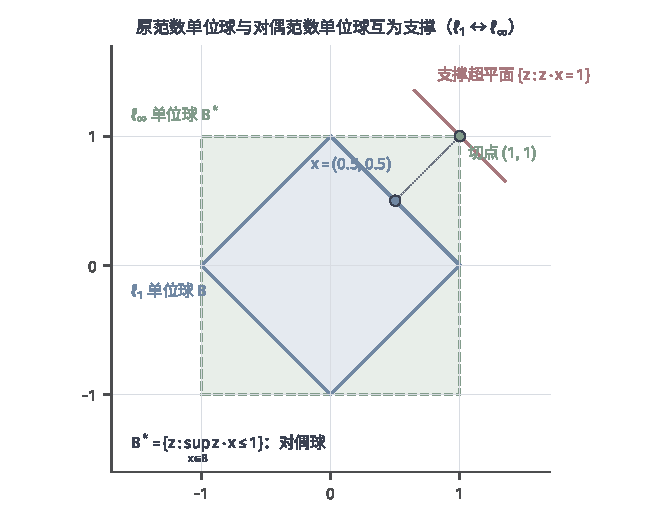
\includegraphics[width=112mm]{figures/00-shared/mathematical-preliminaries-upper/02-linear-spaces/matplotlib/ls-dual-norm-unit-ball/ls-dual-norm-unit-ball.pdf}
  \caption{对偶范数的几何：在原范数单位球$\lVert\bm r\rVert\leq1$上求线性读取$\bm z^\top\bm r$的最大值。左：原单位球（灰色）与读取方向$\bm z$；右：支撑直线最后接触单位球处给出$\lVert\bm z\rVert_*=\max_{\lVert\bm r\rVert\leq1}|\bm z^\top\bm r|$。对偶单位球（虚线）与原单位球互为极体，为解析教学例。}
  \label{fig:ls-dual-norm-unit-ball}
\end{figure}

对$\ell_p$范数，
\begin{equation}
\begin{gathered}
(\lVert\cdot\rVert_p)_*=\lVert\cdot\rVert_q\\
\frac1p+\frac1q=1,
\end{gathered}
\label{eq:linear-algebra-lp-duality}
\end{equation}
并且由齐次性，对$\rho\geq0$有
\begin{equation}
 \max_{\lVert\bm r\rVert_p\leq\rho}|\bm z^\top\bm r|
 =\rho\lVert\bm z\rVert_q.
 \label{eq:linear-algebra-linear-perturbation-duality}
\end{equation}
本节的Hölder不等式（定理~\ref{thm:linear-algebra-holder}）给出$\ell_p$单位球上的上界$\lVert\bm z\rVert_q$。这个上界可以达到：$1<p<\infty$且$\bm z\neq\bm0$时取$r_j=|z_j|^{q-1}\operatorname{sgn}(z_j)/\lVert\bm z\rVert_q^{q-1}$；$\bm z=\bm0$时上界为零，任取可行输入即可。$p=1$时把单位预算全部放在$|z_j|$最大的坐标上；$p=\infty$时逐坐标取$r_j=\operatorname{sgn}(z_j)$。下面固定一个读取，比较三种误差预算。
\begin{example}[同一读取在三种误差预算下的最大变化]
\label{ex:ls-dual-norm-three-budgets}
给定：读取方向$\bm z=(2,-1)^\top$，即读取$\bm z^\top\bm r=2r_1-r_2$。

计算：在$\ell_1$单位球上，把单位预算全部放在$|z_j|$最大的第一个坐标，$\bm r=(1,0)^\top$给出最大值$\lVert\bm z\rVert_\infty=2$。在$\ell_2$单位球上，取$\bm r=\bm z/\lVert\bm z\rVert_2=(2,-1)^\top/\sqrt5$，最大值为$\lVert\bm z\rVert_2=\sqrt5$。在$\ell_\infty$单位球上，逐坐标取$r_j=\operatorname{sgn}(z_j)$，$\bm r=(1,-1)^\top$给出最大值$\lVert\bm z\rVert_1=3$。若误差预算为$|r_j|\leq0.01$，在式~\eqref{eq:linear-algebra-linear-perturbation-duality}中取$p=\infty$、$\rho=0.01$，最大变化为$0.01\cdot(2+1)=0.03$，由$\bm r=(0.01,-0.01)^\top$达到。

结论：同一次读取在$\ell_1$、$\ell_2$、$\ell_\infty$单位球上的最大值依次为$2$、$\sqrt5$、$3$；改变误差预算的形状，最坏方向和最大变化都随之改变。
\end{example}
图~\ref{fig:linear-algebra-dual-unit-balls}画出这三种情形下的最坏方向。
\begin{figure*}[htbp]
  \centering
  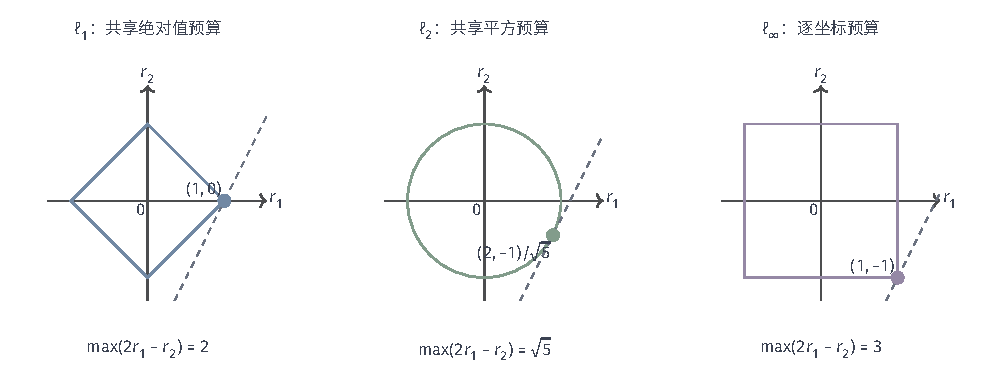
\includegraphics[width=168.998mm]{figures/00-shared/mathematical-preliminaries-upper/02-linear-spaces/tikz/linear-algebra-dual-unit-balls/figure.pdf}
  \caption{同一线性读取$2r_1-r_2$在$\ell_1$、$\ell_2$、$\ell_\infty$单位球上的最大值依次为$2$、$\sqrt5$、$3$。虚线为最后接触可行集的支撑直线，点为最大化方向。三图坐标尺度相同，均为解析教学例；改变允许误差的形状会改变误差常数。}
  \label{fig:linear-algebra-dual-unit-balls}
\end{figure*}

误差预算按$\ell_\infty$给出时，读取方向要按$\ell_1$计量；预算按$\ell_2$给出时，读取方向仍按$\ell_2$计量。所以讨论“输入误差最多引起多大输出误差”时，必须先说清误差用哪种范数度量。

\subsection{商范数}
\label{sec:ls-quotient-norms}

有限维子空间的闭性还可以用来为商空间定义范数。第~\ref{sec:ls-quotient-spaces}节的商空间$V/U$把相差$U$中向量的点看成同一个类$\bm x+U$，那里只建立了线性结构。同一类中各点到$U$的距离相同：若$\bm x'=\bm x+\bm u_0$，$\bm u_0\in U$，则$\bm u$遍历$U$时$\bm u-\bm u_0$也遍历$U$，所以$d(\bm x',U)=d(\bm x,U)$。因此可以把这个距离当作类的大小，称为商范数
\[
 \lVert\bm x+U\rVert_{V/U}=d(\bm x,U)=\inf_{\bm u\in U}\lVert\bm x-\bm u\rVert .
\]
它满足范数的三条要求。三角不等式：对任意$\bm u,\bm u'\in U$，$d(\bm x+\bm y,U)\leq\lVert(\bm x-\bm u)+(\bm y-\bm u')\rVert\leq\lVert\bm x-\bm u\rVert+\lVert\bm y-\bm u'\rVert$，再对$\bm u,\bm u'$分别取下确界。齐次性：$c\neq0$时$cU=U$，所以$d(c\bm x,U)=|c|\,d(\bm x,U)$；$c=0$时两边都为零。正定性要求$d(\bm x,U)=0$只在$\bm x+U=U$即$\bm x\in U$时发生，这正是上面的闭性结论。

\paragraph{一般范数下的最近点}
距离$d(\bm y,U)$定义为下确界，它总能取到吗？由$d(\bm y,U)\leq\lVert\bm y-\bm0\rVert=\lVert\bm y\rVert$，而$\lVert\bm u\rVert>2\lVert\bm y\rVert$时$\lVert\bm y-\bm u\rVert\geq\lVert\bm u\rVert-\lVert\bm y\rVert>\lVert\bm y\rVert$，所以只需在$K=\{\bm u\in U:\lVert\bm u\rVert\leq2\lVert\bm y\rVert\}$上找最小值。由子空间闭性，$K$是闭有界集，按“收敛与连续性”一段的最值论证，连续函数$\bm u\mapsto\lVert\bm y-\bm u\rVert$在其上取到最小值，所以最近点存在。

唯一性却可能失败。
\begin{example}[反例：$\ell_\infty$范数下最近点不唯一]
\label{ex:ls-linf-nonunique-nearest}
给定：$\mathbb R^2$取$\ell_\infty$范数，子空间$U=\operatorname{span}\{(1,0)^\top\}$，点$\bm y=(0,1)^\top$。

计算：$U$中的点写成$(t,0)^\top$，
\[
 \lVert\bm y-(t,0)^\top\rVert_\infty=\max\{|t|,1\}\geq1,
\]
等号当且仅当$|t|\leq1$时成立。

结论：$d(\bm y,U)=1$，所有满足$|t|\leq1$的点$(t,0)^\top$都是最近点，最近点不唯一。
\end{example}
内积诱导的范数下最近点唯一，并由正规方程算出（第~\ref{sec:ls-subspace-nearest-points}节）。

% 第5章第6节：内积空间（内积与内积空间、Gram矩阵、子空间之间的正交、标准正交基的定义和性质、标准正交基的构建、伴随、完备性与Hilbert空间）。

\section{内积空间与Gram矩阵}
\label{sec:ls-inner-product-spaces}

上一节用范数度量大小，但范数不给出角度：一般范数下谈不上两个方向是否垂直，向子空间的最近点也可能不唯一（示例~\ref{ex:ls-linf-nonunique-nearest}）。第~\ref{chap:linear-operations}章在$\mathbb R^d$上定义了欧氏内积，用逐项相乘再求和完成具体计算。本节提取这种计算的共同规则，在一般线性空间上定义内积。

本节先从内积公理建立长度、夹角与基本不等式，再用Gram矩阵记录一组向量之间的配对。随后两节讨论正交投影、标准正交基、泛函表示与伴随；这些工具主要在有限维空间中构造。

\subsection{内积与内积诱导的范数}
\label{sec:ls-inner-product-definition}

本小节只用内积的公理推出长度、夹角及相关不等式，说明内积空间都是赋范空间，并指出并非每个范数都来自内积。

\paragraph{一般线性空间上的内积}
欧氏内积对每个变量都保持线性组合，交换两个变量不改变结果，向量与自身的配对只在零向量处为零。这些性质只涉及线性运算，因此可以用来定义一般空间上的内积。
\begin{definition}[内积空间]
\label{def:functional-inner-product-space}
\label{def:linear-algebra-inner-product}
设$V$是实线性空间。映射$\langle\cdot,\cdot\rangle:V\times V\to\mathbb R$若对任意$\bm x,\bm y,\bm z\in V$与$a,b\in\mathbb R$满足
\begin{enumerate}
 \item 双线性：$\langle a\bm x+b\bm y,\bm z\rangle=a\langle\bm x,\bm z\rangle+b\langle\bm y,\bm z\rangle$，且$\langle\bm z,a\bm x+b\bm y\rangle=a\langle\bm z,\bm x\rangle+b\langle\bm z,\bm y\rangle$；
 \item 对称性：$\langle\bm x,\bm y\rangle=\langle\bm y,\bm x\rangle$；
 \item 正定性：$\langle\bm x,\bm x\rangle\geq0$，且$\langle\bm x,\bm x\rangle=0$当且仅当$\bm x=\bm0$，
\end{enumerate}
就称为$V$上的\term{内积}（inner product）；配备内积的线性空间$(V,\langle\cdot,\cdot\rangle)$称为\term{内积空间}（inner-product space）。
\end{definition}
\paragraph{欧氏内积的公理检验}

下面逐条验证欧氏内积满足定义~\ref{def:linear-algebra-inner-product}的三条公理。

设$\bm x,\bm y,\bm z\in\mathbb R^d$，$a,b\in\mathbb R$。

先看对称性。
\[
 \langle\bm x,\bm y\rangle=\langle\bm y,\bm x\rangle,
\]
因为每一项$x_jy_j=y_jx_j$。

再看双线性。
\[
 \langle a\bm x+b\bm z,\bm y\rangle=a\langle\bm x,\bm y\rangle+b\langle\bm z,\bm y\rangle,
\]
由有限和的运算法则$\sum_j(ax_j+bz_j)y_j=a\sum_jx_jy_j+b\sum_jz_jy_j$得到；再由对称性，对第二个变量同样成立。

最后看正定性。
\[
 \begin{gathered}
 \langle\bm x,\bm x\rangle\geq0,\\
 \langle\bm x,\bm x\rangle=0\iff\bm x=\bm0,
 \end{gathered}
\]
因为$\langle\bm x,\bm x\rangle=\sum_jx_j^2$，而非负数之和为零时每一项都为零。


Frobenius内积满足定义~\ref{def:linear-algebra-inner-product}的三条公理：它对两个变量分别线性；交换两个矩阵不改变各项乘积，因而对称；$\langle\bm A,\bm A\rangle_{\mathrm F}=\sum_{i,j}a_{i,j}^2$非负，并且只在$\bm A=\bm0$时为零。这正是把$mn$个元素看作坐标时欧氏内积的三条性质，所以它确实是同形矩阵上的一个内积，下面从公理推出的一般结论对它同样成立。

标准内积之外，一般空间上可以有各种内积。下面在$P_1$上规定一个只看两点取值的内积，后面的算例会反复用到它。
\begin{example}[只看两点取值的内积]
\label{ex:ls-two-point-inner-product}
给定：$P_1$上的规则$\langle f,g\rangle=f(0)g(0)+f(1)g(1)$。

验证：右端对$f$与对$g$分别是线性的，交换$f,g$也不改变右端，所以双线性与对称性成立。$\langle f,f\rangle=f(0)^2+f(1)^2\geq0$；若它为零，则$f(0)=f(1)=0$，对$f=a+bt$即$a=0$、$a+b=0$，故$f=0$，正定性也成立。

结论：这一规则是$P_1$上的内积。它只看函数在$t=0,1$两点的取值，与系数向量$(a,b)^\top$的欧氏内积不同：例如$\langle1,t\rangle=1\cdot0+1\cdot1=1$，而$1$与$t$的系数向量$(1,0)^\top$、$(0,1)^\top$的欧氏内积为零。
\end{example}

\paragraph{长度与勾股定理}
与$\mathbb R^d$中一样，内积给出长度$\lVert\bm v\rVert=\sqrt{\langle\bm v,\bm v\rangle}$；$\langle\bm x,\bm y\rangle=0$时称$\bm x,\bm y$正交。正交的两个向量满足勾股定理：展开$\lVert\bm x+\bm y\rVert^2=\lVert\bm x\rVert^2+2\langle\bm x,\bm y\rangle+\lVert\bm y\rVert^2$，交叉项为零，得$\lVert\bm x+\bm y\rVert^2=\lVert\bm x\rVert^2+\lVert\bm y\rVert^2$。

\paragraph{Cauchy--Schwarz不等式}
平面上两个非零向量的夹角$\theta$满足
\[
 \langle\bm x,\bm y\rangle=\lVert\bm x\rVert\,\lVert\bm y\rVert\cos\theta.
\]
要在一般内积空间中反过来用这个关系定义夹角，须先保证内积除以两个长度之积以后总落在$[-1,1]$中。
\begin{theorem}[Cauchy--Schwarz不等式]
\label{thm:linear-algebra-cauchy-schwarz}
对任一内积及其长度，任意向量$\bm x,\bm y$满足
\begin{equation}
 |\langle\bm x,\bm y\rangle|\leq\lVert\bm x\rVert\,\lVert\bm y\rVert,
 \label{eq:prelim-cauchy-schwarz}
\end{equation}
等号成立当且仅当其中一个向量是另一个向量的实数倍。
\end{theorem}
\begin{proof}
$\bm y=\bm0$时两边都为零。否则对任意实数$s$，向量$\bm x-s\bm y$的长度平方非负；按内积的对称性与双线性展开，
\[
 0\leq\lVert\bm x-s\bm y\rVert^2
 =\lVert\bm x\rVert^2-2s\langle\bm x,\bm y\rangle+s^2\lVert\bm y\rVert^2.
\]
右侧是$s$的二次函数，二次项系数为正，取顶点$s=\langle\bm x,\bm y\rangle/\lVert\bm y\rVert^2$时最小，此时右侧化为$\lVert\bm x\rVert^2-\langle\bm x,\bm y\rangle^2/\lVert\bm y\rVert^2$。它非负，两边乘以$\lVert\bm y\rVert^2$再开平方，即得不等式。$\bm y\neq\bm0$时，等号成立当且仅当对这个$s$有$\bm x-s\bm y=\bm0$，即$\bm x$是$\bm y$的实数倍；连同$\bm y=\bm0$的情形即得等号条件。
\end{proof}
证明只用了内积的三条公理，所以不等式对每一种内积都成立。在$\mathbb R^d$的标准内积下，它就是$p=q=2$的Hölder不等式（定理~\ref{thm:linear-algebra-holder}）；对Frobenius内积，它给出$|\langle\bm A,\bm B\rangle_{\mathrm F}|\leq\lVert\bm A\rVert_{\mathrm F}\lVert\bm B\rVert_{\mathrm F}$。

\paragraph{三角不等式}
内积给出的长度是否满足定义~\ref{def:ls-normed-space}中范数的三条要求？正定性直接来自内积的正定性，齐次性来自$\langle c\bm x,c\bm x\rangle=c^2\langle\bm x,\bm x\rangle$；需要证明的是三角不等式，Cauchy--Schwarz不等式正好控制展开式中的交叉项。
\begin{theorem}[内积诱导长度的三角不等式]
\label{thm:ls-inner-product-triangle}
设$V$是内积空间，$\lVert\bm v\rVert=\sqrt{\langle\bm v,\bm v\rangle}$，则对任意$\bm x,\bm y\in V$，
\[
 \lVert\bm x+\bm y\rVert\leq\lVert\bm x\rVert+\lVert\bm y\rVert,
\]
等号成立当且仅当其中一个向量是另一个向量的非负实数倍。
\end{theorem}
\begin{proof}
按双线性与对称性展开平方，再对交叉项用$\langle\bm x,\bm y\rangle\leq|\langle\bm x,\bm y\rangle|$与Cauchy--Schwarz不等式~\eqref{eq:prelim-cauchy-schwarz}：
\[
 \begin{aligned}
 \lVert\bm x+\bm y\rVert^2
 &=\lVert\bm x\rVert^2+2\langle\bm x,\bm y\rangle+\lVert\bm y\rVert^2\\
 &\leq\lVert\bm x\rVert^2+2\lVert\bm x\rVert\lVert\bm y\rVert+\lVert\bm y\rVert^2\\
 &=(\lVert\bm x\rVert+\lVert\bm y\rVert)^2.
 \end{aligned}
\]
两边都非负，开平方即得不等式。等号成立当且仅当$\langle\bm x,\bm y\rangle=\lVert\bm x\rVert\,\lVert\bm y\rVert$。若$\bm y=\bm0$，结论显然；若$\bm y\neq\bm0$，由Cauchy--Schwarz不等式的等号条件，$\bm x=s\bm y$，代入得$s\lVert\bm y\rVert^2=|s|\,\lVert\bm y\rVert^2$，即$s\geq0$。反过来，$\bm x=s\bm y$且$s\geq0$时两侧都等于$(1+s)\lVert\bm y\rVert$。
\end{proof}
于是内积给出的长度满足范数的三条要求，每个内积空间都是赋范空间，第~\ref{sec:ls-normed-spaces}节关于收敛与完备性的讨论都适用于它。

\paragraph{平行四边形恒等式}
欧氏范数由内积给出，还满足\term{平行四边形恒等式}。一般范数未必满足这条等式。几何上，它表示平行四边形两条对角线长度的平方和等于四条边长度的平方和。
\begin{theorem}[平行四边形恒等式]
\label{thm:linear-algebra-parallelogram}
设$V$是实内积空间，$\bm x,\bm y\in V$，以该内积诱导的范数计量长度，则
\begin{equation}
 \lVert\bm x+\bm y\rVert^2+\lVert\bm x-\bm y\rVert^2
 =2\lVert\bm x\rVert^2+2\lVert\bm y\rVert^2.
 \label{eq:functional-parallelogram-identity}
\end{equation}
欧氏范数是这一结论的特例。
\end{theorem}
\begin{proof}
记$\lVert\bm u\rVert^2=\langle\bm u,\bm u\rangle$。由内积的双线性和对称性，分别展开和向量与差向量的长度平方：
\[
 \begin{aligned}
 \lVert\bm x+\bm y\rVert^2
 &=\lVert\bm x\rVert^2+2\langle\bm x,\bm y\rangle+\lVert\bm y\rVert^2,\\
 \lVert\bm x-\bm y\rVert^2
 &=\lVert\bm x\rVert^2-2\langle\bm x,\bm y\rangle+\lVert\bm y\rVert^2.
 \end{aligned}
\]
两式相加，交叉项相互抵消，得到所需恒等式。证明只用了内积公理，因此既适用于欧氏内积，也适用于定义~\ref{def:linear-algebra-inner-product}中的任一实内积。
\end{proof}

反过来，恒等式可以检验一个范数是否来自内积：只要某个范数在一对向量上使恒等式两侧不等，它就不可能由任何内积给出。下面的反例用这个办法检验$\ell_1$与$\ell_\infty$范数。
\begin{example}[反例：$\ell_1$与$\ell_\infty$范数不来自内积]
\label{ex:ls-l1-linf-not-inner-product}
给定：$\mathbb R^2$中的$\bm x=\bm e_1$、$\bm y=\bm e_2$，于是$\bm x+\bm y=(1,1)^\top$，$\bm x-\bm y=(1,-1)^\top$。
计算：对$\ell_1$范数，
\[
 \begin{gathered}
 \lVert\bm x+\bm y\rVert_1^2+\lVert\bm x-\bm y\rVert_1^2=2^2+2^2=8,\\
 2\lVert\bm x\rVert_1^2+2\lVert\bm y\rVert_1^2=2\cdot1^2+2\cdot1^2=4;
 \end{gathered}
\]
对$\ell_\infty$范数，
\[
 \begin{gathered}
 \lVert\bm x+\bm y\rVert_\infty^2+\lVert\bm x-\bm y\rVert_\infty^2=1^2+1^2=2,\\
 2\lVert\bm x\rVert_\infty^2+2\lVert\bm y\rVert_\infty^2=4.
 \end{gathered}
\]
结论：两种范数都使恒等式两侧不等。所以不存在内积使$\lVert\bm x\rVert_1=\sqrt{\langle\bm x,\bm x\rangle}$对一切$\bm x$成立，$\ell_\infty$范数同样不是由内积给出的长度。
\end{example}

内积还可由它诱导的范数恢复。在实空间中，分别展开两个平方并相减，得到极化恒等式
\[
 \langle x,y\rangle=\frac14\bigl(\|x+y\|^2-\|x-y\|^2\bigr).
\]
因此两个实内积若给出同一个范数，就必相同。这也说明平行四边形恒等式不是任意范数的自动性质，而是内积几何对长度的约束。

\paragraph{夹角}
由Cauchy--Schwarz不等式，非零向量的夹角$\theta\in[0,\pi]$可以由
\[
 \cos\theta=\frac{\langle\bm x,\bm y\rangle}{\lVert\bm x\rVert\,\lVert\bm y\rVert}
 =\left\langle\frac{\bm x}{\lVert\bm x\rVert},\frac{\bm y}{\lVert\bm y\rVert}\right\rangle
\]
定义。第二种写法说明，夹角只比较方向：先把两个向量各自归一化为单位向量，再取内积；$\bm x$与$c\bm x$（$c>0$）给出同一个方向。正交恰好对应$\theta=\pi/2$，这就是把正交称为垂直的理由；等号条件说明$\cos\theta=\pm1$恰好对应两个向量共线。夹角要求长度来自同一个内积，一边用$\ell_2$、一边用$\ell_1$计量长度时，比值没有几何意义。

回到第~\ref{chap:linear-operations}章两个特征的取值向量，看它们的夹角。
\begin{example}[贯穿例两列的夹角]
\label{ex:ls-nearly-collinear-angle}
给定：$\bm c_1=(1,1,1)^\top$与$\bm c_2=(1,1+\varepsilon,1-\varepsilon)^\top$，取欧氏内积。

计算：$\langle\bm c_1,\bm c_2\rangle=1+(1+\varepsilon)+(1-\varepsilon)=3$，$\lVert\bm c_1\rVert_2^2=3$，$\lVert\bm c_2\rVert_2^2=1+(1+\varepsilon)^2+(1-\varepsilon)^2=3+2\varepsilon^2$，所以
\begin{equation}
 \cos\theta_\varepsilon=\frac{3}{\sqrt3\,\sqrt{3+2\varepsilon^2}}
 =\frac{1}{\sqrt{1+2\varepsilon^2/3}}\longrightarrow1\qquad(\varepsilon\to0).
 \label{eq:linear-algebra-nearly-collinear-angle}
\end{equation}
$\varepsilon=0.1$时$\cos\theta_\varepsilon\approx0.9967$，夹角约$4.7^\circ$；$\varepsilon=0.01$时$\cos\theta_\varepsilon\approx0.99997$，夹角不到$0.5^\circ$。

结论：$\varepsilon\to0$时两列的夹角趋于零；当$\varepsilon$非零且很小时，两个向量不重合，却几乎同向。
\end{example}
两个向量不重合却几乎同向，称为\term{近共线}（nearly collinear）。“近”指作为$\mathbb R^3$中向量的两列夹角很小，不是说各个样本点彼此接近。夹角也依赖所用的内积，换一种内积，同两个向量的夹角会改变。

平行四边形恒等式及其后的反例已经说明，并非每个范数都来自内积。因此，一般范数只能度量大小，不能直接使用这里的公式定义夹角。

\paragraph{复内积的约定}
前面的定义和夹角讨论都针对实空间。复空间中，若两个槽位都按复数线性且满足实数式的对称性，那么$\langle\mathrm i\bm x,\mathrm i\bm x\rangle=-\langle\bm x,\bm x\rangle$，无法对非零向量保持正定。因此复内积采用不同约定：对第一个变量共轭线性，对第二个变量线性，并满足$\langle\bm x,\bm y\rangle=\overline{\langle\bm y,\bm x\rangle}$。标准例子是$\langle\bm x,\bm y\rangle=\bm x^*\bm y$，其中$\bm x^*$表示共轭转置；仍要求$\langle\bm x,\bm x\rangle>0$对非零$\bm x$成立。

复内积同样满足Cauchy--Schwarz不等式。若$\bm y\ne\bm0$，在$\|\bm x-\alpha\bm y\|^2\geq0$中取$\alpha=\langle\bm y,\bm x\rangle/\|\bm y\|^2$，展开可得$|\langle\bm x,\bm y\rangle|^2\leq\|\bm x\|^2\|\bm y\|^2$。因此平方根仍给出范数；但复内积可能不是实数，实空间用余弦定义夹角的公式不能直接照搬。下面的具体证明继续使用实内积，复情形需要把转置相应改为共轭转置。

\paragraph{有限维完备性与Hilbert空间}
\label{sec:ls-hilbert-spaces}
内积诱导的范数使内积空间成为赋范空间。若这个范数下的每个柯西列都收敛到空间内的元素，就称它为\term{Hilbert空间}（Hilbert space，也译作希尔伯特空间）。由定理~\ref{thm:ls-finite-dimensional-complete}，有限维内积空间都满足这一条件。

这里的完备性来自有限个坐标和标量完备性，不能直接推广到无限维。无限正交级数、闭子空间上的投影以及连续泛函的表示，都需要另行核对收敛、闭性和连续性；这些结论在\BookChapterRef{chap:functional-analysis-and-approximation}{第~\ref{chap:functional-analysis-and-approximation}章}建立。

\subsection{Gram矩阵}
\label{sec:ls-gram-psd}

加权内积由一个正定矩阵给出。反过来看，一组向量的全部两两内积也排成一个对称矩阵。本小节说明，这样的矩阵恰好是全部半正定矩阵，从中可以读出这组向量是否线性无关、是否两两正交；最后用基的Gram矩阵写出一般内积空间在坐标下的计算公式。

\paragraph{正定矩阵与半正定矩阵}
$n$阶对称矩阵$\bm M$与向量$\bm x\in\mathbb R^n$给出一个数
\[
 q(\bm x)=\sum_{i=1}^n\sum_{j=1}^n m_{i,j}x_ix_j,
\]
称为$\bm M$的二次型；用矩阵乘法，它写作$\bm x^\top\bm M\bm x$。

若对每个非零$\bm x$都有$q(\bm x)>0$，就称$\bm M$\term{正定}（positive definite），记作$\bm M\succ\bm0$；若只保证$q(\bm x)\geq0$对一切$\bm x$成立，就称$\bm M$\term{半正定}（positive semidefinite），记作$\bm M\succeq\bm0$。对两个同阶对称矩阵，$\bm M\succeq\bm N$表示$\bm M-\bm N\succeq\bm0$，即$\bm M$的二次型处处不小于$\bm N$的二次型；它比较的是两个二次型，不是逐个元素。

判断正定性，要看二次型能否在某个非零向量处取到零或负值。下面用配方比较两个二阶矩阵。
\begin{example}[用配方区分正定与半正定]
\label{ex:ls-pd-psd-completing-square}
给定：$\bm M=\left[\begin{smallmatrix}4&2\\2&2\end{smallmatrix}\right]$，$\bm N=\left[\begin{smallmatrix}1&1\\1&1\end{smallmatrix}\right]$。
计算：两者的二次型配方为
\[
 \begin{aligned}
 q_{\bm M}(\bm x)&=4x_1^2+4x_1x_2+2x_2^2=(2x_1+x_2)^2+x_2^2,\\
 q_{\bm N}(\bm x)&=x_1^2+2x_1x_2+x_2^2=(x_1+x_2)^2.
 \end{aligned}
\]
$q_{\bm M}$是两个平方之和，只在$2x_1+x_2=0$且$x_2=0$，即$\bm x=\bm0$时为零。$q_{\bm N}$处处非负，但在非零向量$\bm x=(1,-1)^\top$处为零。
结论：$\bm M\succ\bm0$；$\bm N\succeq\bm0$，但$\bm N$不是正定矩阵。
\end{example}

对角矩阵的二次型是$\sum_id_ix_i^2$。若全部$d_i>0$，每个非零$\bm x$都使它为正；若某个$d_i\leq0$，取$\bm x=\bm e_i$就得到$q(\bm e_i)=d_i\leq0$。所以对角矩阵正定当且仅当全部$d_i>0$，例如$\bm I_n\succ\bm0$。

正定性要对全部非零向量检查，只看元素的符号并不够，下面的反例说明这一点。
\begin{example}[反例：元素全为正的对称矩阵未必正定]
\label{ex:ls-positive-entries-not-pd}
给定：$\bm M=\left[\begin{smallmatrix}1&2\\2&1\end{smallmatrix}\right]$，四个元素都为正。
计算：它的二次型为$q(\bm x)=x_1^2+4x_1x_2+x_2^2$。取$\bm x=(1,-1)^\top$，
\[
 q(\bm x)=1^2+4\cdot1\cdot(-1)+(-1)^2=-2.
\]
结论：$q(\bm x)<0$，所以$\bm M$不是正定矩阵，也不是半正定矩阵。
\end{example}


\paragraph{Gram矩阵}
\phantomsection
\label{sec:ls-gram-orthogonality}
正交是两个向量之间的关系。一组向量$\bm b_1,\ldots,\bm b_r$之间有$r^2$个配对值，怎样一次记录它们，并从中读出这组向量是否两两正交、某个线性组合会不会退化为零？
\begin{definition}[有限向量族的Gram矩阵]
\label{def:linear-algebra-gram-matrix}
设$\bm b_1,\ldots,\bm b_r$是内积空间$V$中的向量。以$g_{i,j}=\langle\bm b_i,\bm b_j\rangle$为元素的$r$阶矩阵$\bm G$称为它们的\term{Gram矩阵}（Gram matrix）。在$\mathbb R^m$中，若$\bm B$以这些向量为列，则欧氏内积下$\bm G=\bm B^\top\bm B$，加权内积$\langle\cdot,\cdot\rangle_{\bm M}$下$\bm G=\bm B^\top\bm M\bm B$。
\end{definition}
矩阵形式来自乘积的元素公式：$(\bm B^\top\bm B)_{i,j}$是$\bm B^\top$的第$i$行（即$\bm b_i^\top$）与$\bm B$的第$j$列相乘。由内积的对称性，$\bm G$是对称矩阵。

对任意系数向量$\bm a\in\mathbb R^r$，按双线性展开得
\[
 \bm a^\top\bm G\bm a=\sum_{i,j}a_ia_j\langle\bm b_i,\bm b_j\rangle=\Bigl\lVert\sum_j a_j\bm b_j\Bigr\rVert^2\geq0,
\]
所以Gram矩阵半正定。它正定，当且仅当只有全零系数使线性组合$\sum_ja_j\bm b_j$为零，即这组向量线性无关（第~\ref{sec:ls-linear-dependence}节）：组合为零时平方长度为零，组合非零时平方长度为正。

正定的Gram矩阵可逆：若$\bm G\bm a=\bm0$，则$\bm a^\top\bm G\bm a=0$，从而$\bm a=\bm0$，零空间为零（第~\ref{sec:ls-injective-surjective-invertible}节）。正交性也写在Gram矩阵里：$\bm G$是对角矩阵恰好表示这组向量两两正交，$\bm G=\bm I_r$则表示它们两两正交且长度都为$1$。图~\ref{fig:ls-gram-matrix-coefficients}把两条向量的两两内积排成数表。
\begin{figure}[!htb]
  \centering
  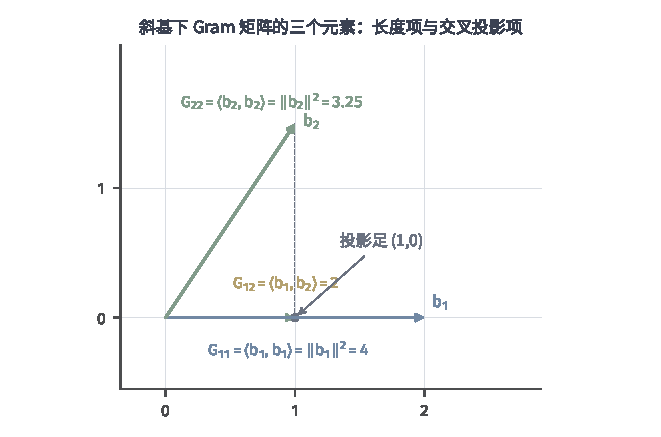
\includegraphics[width=112mm]{figures/00-shared/mathematical-preliminaries-upper/02-linear-spaces/matplotlib/ls-gram-matrix-coefficients/ls-gram-matrix-coefficients.pdf}
  \caption{Gram矩阵把一组基向量的两两内积排成数表。左：平面上两条不垂直的基向量$\bm b_1,\bm b_2$及其夹角；右：$G_{i,j}=\langle\bm b_i,\bm b_j\rangle$构成的$2\times2$Gram矩阵，对角元为各向量长度平方，非对角元为夹角投影。基越接近正交，非对角元越接近零；两向量共线时，某个非零组合的平方长度为零，Gram矩阵不再正定。向量与矩阵均为解析教学例。}
  \label{fig:ls-gram-matrix-coefficients}
\end{figure}

近共线在Gram矩阵上怎样表现？
\begin{example}[近共线两列的Gram矩阵]
\label{ex:ls-nearly-collinear-gram}
给定：贯穿例的两列$\bm c_1,\bm c_2$，取欧氏内积。

计算：由示例~\ref{ex:ls-nearly-collinear-angle}中的三个内积，
\[
\begin{gathered}
\bm G=\bm X_\varepsilon^\top\bm X_\varepsilon=\begin{bmatrix}3&3\\3&3+2\varepsilon^2\end{bmatrix}\\
\bm a^\top\bm G\bm a=3(a_1+a_2)^2+2\varepsilon^2a_2^2 .
\end{gathered}
\]
$\varepsilon\neq0$时，二次型只在$a_1=a_2=0$时为零，所以$\bm G$正定。取$\bm a=(1,-1)^\top$，二次型只有$2\varepsilon^2$；对应的组合$\bm c_1-\bm c_2=-\varepsilon\bm q$确实很短。

结论：$\bm G$正定，与两列线性无关一致；但存在系数使二次型接近零。近共线在Gram矩阵上表现为“正定但几乎退化”。
\end{example}

\paragraph{Gram因子定理}
Gram矩阵总是半正定的。反过来，每个半正定矩阵是否都是某组向量的Gram矩阵？关键是把半正定矩阵写成欧氏平方和，这一分解也说明加权配对不必当作新的几何。
\begin{theorem}[半正定矩阵的配方因子]
\label{thm:ls-gram-factor}
设$\bm M\in\mathbb R^{r\times r}$对称半正定，则存在$\bm L\in\mathbb R^{r\times r}$使$\bm M=\bm L^\top\bm L$；若$\bm M$正定，可取$\bm L$可逆。
\end{theorem}
\begin{proof}
对$r$归纳。$r=1$时$\bm M=(m_{1,1})$且$m_{1,1}\geq0$，取$\bm L=(\sqrt{m_{1,1}})$即可。

设$r>1$。若所有对角元都为零，任取$i\neq j$，把$\bm x=\bm e_i+t\bm e_j$代入半正定性：
\[
 0\leq\bm x^\top\bm M\bm x=m_{i,i}+2t\,m_{i,j}+t^2m_{j,j}=2t\,m_{i,j},
\]
对正负$t$同时成立迫使$m_{i,j}=0$，于是$\bm M=\bm0$，取$\bm L=\bm0$。

否则存在正的对角元。取一个置换矩阵$\bm P$把它换到首位（行列同步交换）；$\bm P$的各列是互不相同的标准坐标向量，所以$\bm P^\top\bm P=\bm P\bm P^\top=\bm I$。记
\[
\begin{gathered}
\widetilde{\bm M}=\bm P\bm M\bm P^\top
 =\begin{bmatrix}a&\bm b^\top\\ \bm b&\bm C\end{bmatrix}\\
a>0.
\end{gathered}
\]
$\widetilde{\bm M}$仍对称半正定，因为$\bm x^\top\widetilde{\bm M}\bm x=(\bm P^\top\bm x)^\top\bm M(\bm P^\top\bm x)\geq0$。对第一个变量配方：令$\bm x=(-\bm b^\top\bm u/a,\bm u)$，展开得$\bm x^\top\widetilde{\bm M}\bm x=\bm u^\top(\bm C-\bm b\bm b^\top/a)\bm u\geq0$，故余项$\bm M'=\bm C-\bm b\bm b^\top/a$仍半正定。由归纳假设$\bm M'=\bm L'^\top\bm L'$，取上三角因子
\[
 \widetilde{\bm L}=\begin{bmatrix}\sqrt a&\bm b^\top/\sqrt a\\ \bm0&\bm L'\end{bmatrix},
\]
按分块乘法直接相乘得
\[
 \widetilde{\bm L}^\top\widetilde{\bm L}
 =\begin{bmatrix}a&\bm b^\top\\ \bm b&\bm b\bm b^\top/a+\bm L'^\top\bm L'\end{bmatrix}
 =\widetilde{\bm M}.
\]
换回原矩阵：$\bm M=\bm P^\top\widetilde{\bm M}\bm P=(\widetilde{\bm L}\bm P)^\top(\widetilde{\bm L}\bm P)$，取$\bm L=\widetilde{\bm L}\bm P$即可。

正定时$\bm M'$也正定（上述$\bm x$在$\bm u\neq\bm0$时非零），归纳得$\bm L'$可逆。分块上三角矩阵$\widetilde{\bm L}$的对角块$\sqrt a$与$\bm L'$都可逆，按分块乘法可以直接验证
\[
 \begin{bmatrix}1/\sqrt a&-\bm b^\top\bm L'^{-1}/a\\ \bm0&\bm L'^{-1}\end{bmatrix}
\]
是它的逆，于是$\bm L=\widetilde{\bm L}\bm P$作为可逆矩阵的乘积仍可逆。
\end{proof}
下面对一个二阶正定矩阵按证明的步骤求出因子。
\begin{example}[二阶正定矩阵的配方因子]
\label{ex:ls-gram-factor-two-by-two}
给定：$\bm M=\left[\begin{smallmatrix}4&2\\2&2\end{smallmatrix}\right]$。

计算：首个对角元$a=4>0$，不需要置换；$\bm b=(2)$，余项$\bm M'=2-2^2/4=1$，取$\bm L'=(1)$。按证明中的分块形式，
\[
 \bm L=\begin{bmatrix}\sqrt a&\bm b^\top/\sqrt a\\ 0&\bm L'\end{bmatrix}=\begin{bmatrix}2&1\\0&1\end{bmatrix}.
\]
直接验证：$\bm L^\top\bm L=\left[\begin{smallmatrix}2&0\\1&1\end{smallmatrix}\right]\left[\begin{smallmatrix}2&1\\0&1\end{smallmatrix}\right]=\left[\begin{smallmatrix}4&2\\2&2\end{smallmatrix}\right]=\bm M$。相应地，
\[
 \bm x^\top\bm M\bm x=4x_1^2+4x_1x_2+2x_2^2=(2x_1+x_2)^2+x_2^2 .
\]

结论：$\bm M=\bm L^\top\bm L$，且$\bm L$可逆；二次型被写成两个平方之和。
\end{example}
于是正定矩阵给出的加权长度可写成$\lVert\bm x\rVert_{\bm M}=\lVert\bm L\bm x\rVert_2$：加权内积只是把$\bm x$换成新坐标$\bm L\bm x$再量欧氏长度。证明中的配方步骤就是第~\ref{sec:ls-exact-linear-equations}节Cholesky分解的雏形。

\paragraph{半正定矩阵与Gram矩阵}
Gram矩阵总是半正定的；反过来，每个半正定矩阵都是某组向量的Gram矩阵。由定理~\ref{thm:ls-gram-factor}，半正定的$\bm M$可写成$\bm M=\bm L^\top\bm L$，记$\bm l_i$为$\bm L$的第$i$列，则$m_{i,j}=\bm l_i^\top\bm l_j=\langle\bm l_i,\bm l_j\rangle$，$\bm M$正是$\bm l_1,\ldots,\bm l_r$在欧氏内积下的Gram矩阵。所以“半正定”与“是一组向量的两两内积”说的是同一件事，判断一个矩阵半正定，可以去找这样一组向量。

这一观点给出一个关于逐元素乘积（第~\ref{sec:ls-hadamard-product}节）的结论：两个半正定矩阵的逐元素乘积仍半正定吗？设$\bm A,\bm B$均为$n$阶半正定矩阵。由定理~\ref{thm:ls-gram-factor}，$\bm A=\bm U^\top\bm U$、$\bm B=\bm V^\top\bm V$；记$\bm u_i,\bm v_i$分别为$\bm U,\bm V$的第$i$列，则$A_{i,k}=\langle\bm u_i,\bm u_k\rangle$、$B_{i,k}=\langle\bm v_i,\bm v_k\rangle$。考虑二阶数组$\bm u_1\otimes\bm v_1,\ldots,\bm u_n\otimes\bm v_n$，由Frobenius内积下张量积配对的分离性（第~\ref{sec:ls-tensor-operation-properties}节），它们的Gram矩阵为
\[
 \langle\bm u_i\otimes\bm v_i,\bm u_k\otimes\bm v_k\rangle_{\mathrm F}
 =\langle\bm u_i,\bm u_k\rangle\langle\bm v_i,\bm v_k\rangle
 =A_{i,k}B_{i,k}.
\]
Gram矩阵恒半正定，故逐元素乘积$\bm A\odot\bm B$半正定，这就是\term{Schur乘积}定理（Schur product theorem）。下面用一个二阶例子核对。
\begin{example}[两个半正定矩阵的逐元素乘积]
\label{ex:ls-schur-product}
给定：$\bm A=\bm B=\left[\begin{smallmatrix}1&1\\1&2\end{smallmatrix}\right]$。

计算：$\bm A$的二次型为$x_1^2+2x_1x_2+2x_2^2=(x_1+x_2)^2+x_2^2\geq0$，所以$\bm A$半正定。逐元素乘积及其二次型为
\[
\begin{gathered}
\bm A\odot\bm B=\begin{bmatrix}1&1\\1&4\end{bmatrix}\\
x_1^2+2x_1x_2+4x_2^2=(x_1+x_2)^2+3x_2^2\geq0 .
\end{gathered}
\]

结论：$\bm A\odot\bm B$仍半正定，与Schur乘积定理一致。
\end{example}
核方法中两个核矩阵的逐元素乘积仍是合法的核矩阵，依据就是这一定理。

\paragraph{坐标下的内积}
选定基以后，一般内积空间上的内积也由一张矩阵完全确定，这张矩阵就是基的Gram矩阵。

设$\mathcal B=(\bm b_1,\ldots,\bm b_d)$是$V$的基，$\bm G$是它的Gram矩阵。对$\bm v=\sum_ix_i\bm b_i$、$\bm w=\sum_jy_j\bm b_j$，按双线性展开得
\[
 \langle\bm v,\bm w\rangle=\sum_{i,j}x_iy_j\langle\bm b_i,\bm b_j\rangle=[\bm v]_{\mathcal B}^\top\,\bm G\,[\bm w]_{\mathcal B}.
\]
基线性无关，所以$\bm G$对称正定：在坐标下，任一内积都是以$\bm G$为权重的加权内积。特别地，$\mathbb R^d$上的任一内积在标准基下都是$\bm x^\top\bm G\bm y$，其中$g_{i,j}=\langle\bm e_i,\bm e_j\rangle$；反过来，每个对称正定矩阵都给出一个加权内积。所以$\mathbb R^d$上的内积与$d$阶对称正定矩阵一一对应，欧氏内积对应$\bm I$。下面用示例~\ref{ex:ls-two-point-inner-product}的内积核对坐标公式。
\begin{example}[两点内积的坐标计算]
\label{ex:ls-two-point-inner-product-coordinates}
给定：示例~\ref{ex:ls-two-point-inner-product}中$P_1$上的内积$\langle f,g\rangle=f(0)g(0)+f(1)g(1)$，基$(1,t)$，以及$f=1+t$、$g=1-2t$。

计算：由$\langle1,1\rangle=1\cdot1+1\cdot1=2$、$\langle1,t\rangle=1\cdot0+1\cdot1=1$、$\langle t,t\rangle=0\cdot0+1\cdot1=1$，基的Gram矩阵为
\[
 \bm G=\begin{bmatrix}2&1\\1&1\end{bmatrix}.
\]
按定义，$f$在$t=0,1$处取值$1,2$，$g$取值$1,-1$，所以$\langle f,g\rangle=1\cdot1+2\cdot(-1)=-1$。按坐标，$[f]=(1,1)^\top$、$[g]=(1,-2)^\top$，
\[
 (1,1)\,\bm G\begin{bmatrix}1\\-2\end{bmatrix}=(3,2)\begin{bmatrix}1\\-2\end{bmatrix}=-1 .
\]

结论：两种算法给出同一个内积值$-1$。
\end{example}
若基两两正交且长度为$1$，则$\bm G=\bm I$，内积在坐标下就是欧氏内积；这样的基是第~\ref{sec:ls-orthonormal-bases}节的主题。

\paragraph{其他内积运算}
\phantomsection
\label{sec:ls-weighted-inner-products}
即使在$\mathbb R^d$上，标准内积也不是唯一的选择。各坐标的单位或重要性不同时，可以给不同方向不同的权重：取对称正定矩阵$\bm M$，规定
\begin{equation}
\begin{gathered}
\langle\bm x,\bm y\rangle_{\bm M}=\bm x^\top\bm M\bm y\\
d_{\bm M}(\bm x,\bm y)=\lVert\bm x-\bm y\rVert_{\bm M}=\sqrt{(\bm x-\bm y)^\top\bm M(\bm x-\bm y)}.
\end{gathered}
\label{eq:linear-algebra-mahalanobis-pseudodistance}
\end{equation}
双线性来自矩阵乘法的分配律，对称性来自$\bm M^\top=\bm M$，正定性就是$\bm M$的正定，所以它满足内积的三条公理，称为加权内积，$d_{\bm M}$是它给出的距离。统计中取$\bm M$为协方差矩阵的逆，得到的就是Mahalanobis距离。下面看权重怎样改变同一个点的长度。
\begin{example}[加权内积下的长度]
\label{ex:ls-weighted-length}
给定：$\bm M=\operatorname{diag}(4,1)$与$\bm x=(1,1)^\top$。

计算：$\langle\bm x,\bm y\rangle_{\bm M}=4x_1y_1+x_2y_2$，所以$\lVert\bm x\rVert_{\bm M}^2=4\cdot1+1\cdot1=5$；欧氏长度的平方则为$1+1=2$。

结论：同一个点的加权长度是$\sqrt5$，欧氏长度是$\sqrt2$；权重放大了第一个坐标的作用。
\end{example}
前面的坐标公式已经说明，选定基以后，任一实内积都可以写成这种加权形式。


在复空间中，Gram矩阵的第$(i,j)$项取$\langle v_i,v_j\rangle$，于是$\bm c^*\bm G\bm c=\|\sum_jc_jv_j\|^2$；半正定性与正定性的判别由同一等式得到。逐步配方的证明也保留：分块$\bm G=\left[\begin{smallmatrix}a&\bm b^*\\\bm b&\bm C\end{smallmatrix}\right]$且$a>0$时，分离的平方项为$a|z+\bm b^*\bm y/a|^2$，剩余矩阵是$\bm C-\bm b\bm b^*/a$。若对角全零，取仅两个分量非零且可调相位的向量，半正定性迫使所有非对角元也为零。递推便得到$\bm G=\bm L^*\bm L$，不需要借用后面的谱定理。

换基时，若旧坐标与新坐标满足$\bm x=\bm C\widetilde{\bm x}$，内积配对中的两个坐标都要改变，因此Gram矩阵变为
\[
 \widetilde{\bm G}=\bm C^\top\bm G\bm C.
\]
这称为合同变换，保存同一内积与二次型；相似变换则记录同一算子的换基，两者用途不同。复空间按第一变量共轭线性的约定写成$\langle x,y\rangle=\bm x^*\bm G\bm y$，Gram矩阵Hermitian正定，合同公式中相应使用$\bm C^*$。

\section{正交与投影}

内积给出方向之间的正交关系。本节从正交补开始，将向量分解为子空间中的分量和与它正交的剩余量。

\subsection{正交补与正交分解}
\label{sec:ls-orthogonality}

Gram矩阵记录的是一组向量两两之间是否正交。本小节把正交推广为一个向量与整个子空间的正交，得到由内积唯一确定的补空间，并据此证明四个基本子空间之间的垂直关系。

\paragraph{正交补}
第~\ref{sec:ls-direct-sum}节说明，一个子空间的补空间一般不唯一。有了内积，是否存在一个由“垂直”唯一确定的补空间？设$U$是有限维内积空间$V$的子空间，与$U$中每个向量都正交的向量组成的集合
\[
 U^\perp=\{\bm r\in V:\langle\bm u,\bm r\rangle=0,\ \forall\bm u\in U\}
\]
称为$U$的\term{正交补}（orthogonal complement）。由内积的双线性，$U^\perp$对线性组合封闭，是子空间。要检查$\bm r\in U^\perp$，只需检查它与$U$的一组基逐个正交，因为与基向量都正交的向量与基向量的每个组合也正交。

\paragraph{正交直和}
正交补确实是一个补空间，而且分解可以由Gram矩阵算出。
\begin{lemma}[正交直和]
\label{lem:ls-orthogonal-decomposition}
设$U$是有限维内积空间$V$的子空间，则每个$\bm x\in V$唯一分解为$\bm x=\bm u+\bm r$，其中$\bm u\in U$、$\bm r\in U^\perp$；即$V=U\oplus U^\perp$。
\end{lemma}
\begin{proof}
取$U$的一组基$\bm b_1,\ldots,\bm b_r$，它线性无关，所以Gram矩阵$\bm G$正定，从而可逆。对任意$\bm x$，令$\bm u=\sum_j a_j\bm b_j$，并要求$\bm r=\bm x-\bm u$与每个$\bm b_i$正交，得到系数方程
\[
 \begin{gathered}
\sum_j g_{i,j}a_j=\langle\bm b_i,\bm x\rangle\\
i=1,\ldots,r,
 \end{gathered}
\]
即$\bm G\bm a=(\langle\bm b_i,\bm x\rangle)_i$。可逆的$\bm G$保证系数唯一解出，残差$\bm r$与全部基向量正交，因而落在$U^\perp$。

若$\bm x=\bm u+\bm r=\bm u'+\bm r'$是两种分解，则$\bm u-\bm u'=\bm r'-\bm r$同时属于$U$与$U^\perp$，与自身正交，长度为零，故两种分解相同。
\end{proof}
所以正交补是$U$的一个补空间，并且由内积唯一确定，称$V=U\oplus U^\perp$为正交直和；由维数公式，$\dim U^\perp=\dim V-\dim U$。下面在$\mathbb R^3$中做一次分解。
\begin{example}[向一条直线的正交分解]
\label{ex:ls-orthogonal-decomposition-line}
给定：$\mathbb R^3$取欧氏内积，$U=\operatorname{span}\{\bm c_1\}$，$\bm c_1=(1,1,1)^\top$，$\bm y=(1,1.1,0.9)^\top$。

计算：$U^\perp$由与$\bm c_1$正交的向量组成，即坐标和为零的平面。$U$只有一个基向量，Gram方程只有一个未知数：$\langle\bm c_1,\bm c_1\rangle a=\langle\bm c_1,\bm y\rangle$，即$3a=3$，所以$a=1$。于是
\[
 \begin{gathered}
 \bm u=\bm c_1=(1,1,1)^\top,
 \\
 \bm r=\bm y-\bm u=(0,0.1,-0.1)^\top,
 \end{gathered}
\]
$\bm r$的坐标和为零，确实属于$U^\perp$。

结论：$\bm y=\bm u+\bm r$就是$\bm y$在正交直和$\mathbb R^3=U\oplus U^\perp$中的分解。
\end{example}
这里先得到正交分量的存在与唯一；它为什么是$U$中离$\bm x$最近的点，在下面用标准正交基写出投影后证明。

取两次正交补会回到原来的子空间：$(U^\perp)^\perp=U$。一方面，$U$中每个向量与$U^\perp$中每个向量正交，所以$U\subseteq(U^\perp)^\perp$；另一方面，对$U^\perp$用上面的维数关系，$\dim(U^\perp)^\perp=\dim V-\dim U^\perp=\dim U$。包含且同维，由第~\ref{sec:ls-dimension}节两者相等。

\paragraph{四个基本子空间的正交关系}
示例~\ref{ex:ls-rank-one-four-subspaces}显示，行空间的方向与零空间垂直，列空间的方向与左零空间垂直。现在在$\mathbb R^d$与$\mathbb R^m$上取欧氏内积，证明这对任何矩阵都成立。
\begin{theorem}[四个基本子空间的正交关系]
\label{thm:ls-four-subspaces-orthogonality}
设$\bm A\in\mathbb R^{m\times d}$，$\mathbb R^d$与$\mathbb R^m$取欧氏内积。则
\begin{equation}
\begin{gathered}
\operatorname{null}(\bm A)=\operatorname{range}(\bm A^\top)^\perp\\
\operatorname{null}(\bm A^\top)=\operatorname{range}(\bm A)^\perp,
\end{gathered}
\label{eq:ls-four-subspaces-orthogonality}
\end{equation}
因而有正交直和
\begin{equation}
\begin{gathered}
\mathbb R^d=\operatorname{range}(\bm A^\top)\oplus\operatorname{null}(\bm A)\\
\mathbb R^m=\operatorname{range}(\bm A)\oplus\operatorname{null}(\bm A^\top).
\end{gathered}
\label{eq:ls-four-subspaces-decomposition}
\end{equation}
\end{theorem}
\begin{proof}
由转置的乘积规则（第~\ref{sec:ls-reshaping}节），对任意$\bm x\in\mathbb R^d$、$\bm y\in\mathbb R^m$，
\[
 \langle\bm A\bm x,\bm y\rangle=(\bm A\bm x)^\top\bm y=\bm x^\top(\bm A^\top\bm y)=\langle\bm x,\bm A^\top\bm y\rangle.
\]
$\bm y\in\operatorname{range}(\bm A)^\perp$意味着左端对一切$\bm x$为零，即右端对一切$\bm x$为零；取$\bm x=\bm A^\top\bm y$可见这当且仅当$\bm A^\top\bm y=\bm0$。所以$\operatorname{range}(\bm A)^\perp=\operatorname{null}(\bm A^\top)$。把$\bm A$换成$\bm A^\top$得$\operatorname{range}(\bm A^\top)^\perp=\operatorname{null}(\bm A)$。正交直和由引理~\ref{lem:ls-orthogonal-decomposition}得到。
\end{proof}
两边再取正交补，并用$(U^\perp)^\perp=U$，还得到$\operatorname{null}(\bm A)^\perp=\operatorname{range}(\bm A^\top)$、$\operatorname{null}(\bm A^\top)^\perp=\operatorname{range}(\bm A)$。于是输入空间分成两块互相垂直的部分：零空间是被$\bm A$消去的方向，行空间是真正影响输出的方向；输出空间也分成两块：列空间是可达的输出，左零空间是无论如何都到达不了的方向。

这一定理与第~\ref{sec:ls-kernel-image}节的维数关系相互印证。由正交直和与秩零度定理分别得到
\[
 \begin{gathered}
d=\dim\operatorname{range}(\bm A^\top)+\dim\operatorname{null}(\bm A)\\
d=\operatorname{rank}\bm A+\dim\operatorname{null}(\bm A).
 \end{gathered}
\]
两式比较，又一次得到行秩等于列秩。示例~\ref{ex:ls-rank-one-four-subspaces}中逐项相乘再相加得零的观察，现在由定理得到了解释。

输出端的分解给出方程$\bm A\bm x=\bm b$有解的一个判据：$\bm b\in\operatorname{range}(\bm A)$当且仅当$\bm b$与左零空间中每个向量正交。第~\ref{chap:linear-equations-and-optimization}章判断方程是否有解时会用到这一点。

\subsection{标准正交基}
\label{sec:ls-orthonormal-bases}

正交直和的证明要解Gram方程$\bm G\bm a=(\langle\bm b_i,\bm x\rangle)_i$，坐标下的内积要乘Gram矩阵，示例~\ref{ex:ls-coordinate-instability}还显示，接近共线的基会把小的对象记成很大的系数。这些麻烦都来自基向量之间的相互干扰，即Gram矩阵的非对角元。本小节定义消除这种干扰的基，证明它确实是一组基，再依次给出它下的坐标、它们之间的换基，以及向子空间的正交分解。

\paragraph{标准正交基的定义}
一组向量$\bm q_1,\ldots,\bm q_r$若满足
\[
 \langle\bm q_i,\bm q_j\rangle=\delta_{i,j}=\begin{cases}1,&i=j,\\0,&i\neq j,\end{cases}
\]
即两两正交且长度都为$1$，就称为标准正交组；它的Gram矩阵是$\bm I_r$。张成子空间$U$的标准正交组称为$U$的\term{标准正交基}（orthonormal basis）；$U=V$时就是$V$的标准正交基。

在$\mathbb R^m$中取欧氏内积，把$r$个向量排成$\bm Q\in\mathbb R^{m\times r}$的各列，它们的Gram矩阵是$\bm Q^\top\bm Q$，所以标准正交的条件就是$\bm Q^\top\bm Q=\bm I_r$。$r=m$时$\bm Q$是第~\ref{sec:ls-orthogonal-matrices}节的正交矩阵；$r<m$时$\bm Q^\top\bm Q=\bm I_r$仍成立，但$\bm Q\bm Q^\top$的秩只有$r$，不等于$\bm I_m$，$\bm Q$只有左逆$\bm Q^\top$。

\paragraph{标准正交组构成基}
标准正交组总是线性无关。

设$\sum_jc_j\bm q_j=\bm0$，两边与$\bm q_i$作内积，左边每一项$c_j\langle\bm q_j,\bm q_i\rangle$只在$j=i$时不为零，于是$c_i=0$；$i$任意，所以全部系数为零。同样的论证说明两两正交的非零向量组线性无关，只是最后一步改为由$c_i\langle\bm q_i,\bm q_i\rangle=0$与$\langle\bm q_i,\bm q_i\rangle>0$得$c_i=0$。因此标准正交组是它所张成子空间的一组基；$d$维内积空间中$d$个两两正交的单位向量个数等于维数，自动构成整个空间的标准正交基，不必另行验证张成。$\mathbb R^d$的标准基在欧氏内积下是标准正交基；$\bm q_1=(1,1)^\top/\sqrt2$、$\bm q_2=(1,-1)^\top/\sqrt2$是$\mathbb R^2$的另一组标准正交基。

\paragraph{标准正交基下的坐标}
在标准正交基下，坐标不必解方程。若$\bm v=\sum_jc_j\bm q_j$，两边与$\bm q_i$作内积，右边只剩$c_i$一项，所以
\begin{equation}
 \bm v=\sum_{j=1}^d\langle\bm v,\bm q_j\rangle\,\bm q_j.
 \label{eq:ls-orthonormal-expansion}
\end{equation}
每个系数只与自己的方向有关，增加或删去其他方向都不改变它。坐标下的内积变成欧氏内积：$\langle\bm v,\bm w\rangle=\sum_jc_jd_j$，其中$c_j,d_j$分别是$\bm v,\bm w$的坐标；特别地
\begin{equation}
 \lVert\bm v\rVert^2=\sum_{j=1}^d\langle\bm v,\bm q_j\rangle^2,
 \label{eq:ls-parseval}
\end{equation}
长度的平方等于各坐标的平方和，称为Parseval恒等式，是勾股定理在$d$个互相垂直方向上的推广。下面用平面上的一组标准正交基验证这两点。
\begin{example}[标准正交基下的坐标与Parseval恒等式]
\label{ex:ls-orthonormal-coordinates}
给定：$\mathbb R^2$的标准正交基$\bm q_1=(1,1)^\top/\sqrt2$、$\bm q_2=(1,-1)^\top/\sqrt2$，向量$\bm v=(3,1)^\top$。

计算：由式~\eqref{eq:ls-orthonormal-expansion}，坐标为$\langle\bm v,\bm q_1\rangle=4/\sqrt2=2\sqrt2$与$\langle\bm v,\bm q_2\rangle=2/\sqrt2=\sqrt2$，不必解方程。坐标的平方和为$8+2=10$，而$\lVert\bm v\rVert^2=3^2+1^2=10$。

结论：坐标由内积直接读出，平方和等于长度的平方。
\end{example}
在标准正交基下，坐标的大小如实反映对象的大小，近共线基下“小对象、大系数”的现象不会发生。

\paragraph{正交矩阵}
\phantomsection
\label{sec:ls-orthogonal-matrices}
若$n$阶方阵$\bm Q$的各列都是单位向量，并且两两正交，就称它为\term{正交矩阵}（orthogonal matrix）。单位矩阵和置换矩阵都是正交矩阵，因为它们的列是互不相同的标准坐标向量。

下面检验平面旋转矩阵满足这一定义，并说明只有各列两两正交还不够。
\begin{example}[平面旋转是正交矩阵]
\label{ex:ls-rotation-orthogonal}
给定：任一实数$\phi$对应的平面旋转矩阵
\[
 \bm R_\phi=\begin{bmatrix}\cos\phi&-\sin\phi\\\sin\phi&\cos\phi\end{bmatrix},
\]
以及对角矩阵$\operatorname{diag}(2,1)$。
验证：$\bm R_\phi$两列的长度与内积分别为
\[
 \begin{gathered}
\sqrt{\cos^2\phi+\sin^2\phi}=1\\
\cos\phi\cdot(-\sin\phi)+\sin\phi\cdot\cos\phi=0.
 \end{gathered}
\]$\operatorname{diag}(2,1)$的两列$(2,0)^\top$与$(0,1)^\top$内积为零，但第一列长度为$2$。
结论：$\bm R_\phi$是正交矩阵；$\operatorname{diag}(2,1)$的各列两两正交，却不是正交矩阵，因为正交矩阵还要求每列长度为$1$。
\end{example}
下面从标准正交列出发，统一推导这些性质。


\paragraph{正交矩阵的转置条件}
$n$阶方阵$\bm Q$是正交矩阵，当且仅当
\[
 \bm Q^\top\bm Q=\bm I_n.
\]
$(\bm Q^\top\bm Q)_{i,j}$是$\bm Q$的第$i$列与第$j$列的内积。所以“各列都是单位向量”对应对角元等于$1$，“各列两两正交”对应非对角元等于$0$，两者合起来正是这个矩阵等式。下面用这个条件重新检验示例~\ref{ex:ls-rotation-orthogonal}中的两个矩阵。
\begin{example}[用转置条件检验正交矩阵]
\label{ex:ls-orthogonality-by-transpose}
给定：旋转矩阵$\bm R_\phi$与对角矩阵$\operatorname{diag}(2,1)$。
计算：
\[
 \begin{aligned}
 \bm R_\phi^\top\bm R_\phi
 &=\begin{bmatrix}\cos\phi&\sin\phi\\-\sin\phi&\cos\phi\end{bmatrix}
   \begin{bmatrix}\cos\phi&-\sin\phi\\\sin\phi&\cos\phi\end{bmatrix}\\
 &=\begin{bmatrix}\cos^2\phi+\sin^2\phi&0\\0&\sin^2\phi+\cos^2\phi\end{bmatrix}
 =\bm I_2,\\
 \operatorname{diag}(2,1)^\top\operatorname{diag}(2,1)&=\operatorname{diag}(4,1)\neq\bm I_2.
 \end{aligned}
\]
结论：$\bm R_\phi$满足转置条件，是正交矩阵；$\operatorname{diag}(2,1)$的乘积在$(1,1)$位置为$4\neq1$，对应第一列长度不为$1$。
\end{example}


\paragraph{正交矩阵保持内积}
\[
 \langle\bm Q\bm x,\bm Q\bm y\rangle=\langle\bm x,\bm y\rangle\qquad(\bm Q\text{为正交矩阵}).
\]
由内积中的转置与上一条，$\langle\bm Q\bm x,\bm Q\bm y\rangle=\langle\bm x,\bm Q^\top\bm Q\bm y\rangle=\langle\bm x,\bm y\rangle$。特别地，正交矩阵把两两正交的向量仍送到两两正交的向量。



\paragraph{正交矩阵的乘法}
若$\bm Q_1,\bm Q_2$是$n$阶正交矩阵，则
\[
 (\bm Q_1\bm Q_2)^\top(\bm Q_1\bm Q_2)=\bm Q_2^\top\bm Q_1^\top\bm Q_1\bm Q_2=\bm Q_2^\top\bm Q_2=\bm I_n,
\]
由正交矩阵的转置条件，$\bm Q_1\bm Q_2$仍是正交矩阵。下面的例子显示，两个平面旋转的乘积不仅是正交矩阵，而且仍是旋转。
\begin{example}[两个平面旋转的乘积]
\label{ex:ls-rotation-composition}
给定：旋转矩阵$\bm R_\phi$与$\bm R_\psi$。
计算：直接相乘，再用和角公式$\cos(\phi+\psi)=\cos\phi\cos\psi-\sin\phi\sin\psi$与$\sin(\phi+\psi)=\sin\phi\cos\psi+\cos\phi\sin\psi$，
\[
 \begin{aligned}
 \bm R_\phi\bm R_\psi
 &=\begin{bmatrix}\cos\phi\cos\psi-\sin\phi\sin\psi&-\cos\phi\sin\psi-\sin\phi\cos\psi\\\sin\phi\cos\psi+\cos\phi\sin\psi&-\sin\phi\sin\psi+\cos\phi\cos\psi\end{bmatrix}\\
 &=\bm R_{\phi+\psi}.
 \end{aligned}
\]
结论：先转$\psi$角、再转$\phi$角，等于一次转$\phi+\psi$角；乘积是正交矩阵，与上面的一般结论一致。
\end{example}


\paragraph{正交矩阵的逆}
\[
\begin{gathered}
\bm Q^{-1}=\bm Q^\top\\
\bm Q\bm Q^\top=\bm I_n\qquad(\bm Q\text{为正交矩阵}).
\end{gathered}
\]
正交矩阵的转置条件$\bm Q^\top\bm Q=\bm I_n$只说明$\bm Q^\top$是$\bm Q$的左逆。方阵只要有一侧的逆就可逆，而且这个单侧逆就是逆矩阵；这一点的证明要用到行列式，放在第~\ref{sec:ls-square-one-sided-inverse}节。由此$\bm Q^{-1}=\bm Q^\top$，另一侧的乘积$\bm Q\bm Q^\top$也等于$\bm I_n$。

$\bm Q\bm Q^\top$的$(i,j)$元是$\bm Q$的第$i$行与第$j$行的内积，所以正交矩阵的各行同样两两正交且长度为$1$，求逆只需转置。又因$(\bm Q^\top)^\top\bm Q^\top=\bm Q\bm Q^\top=\bm I_n$，由转置条件，$\bm Q^{-1}=\bm Q^\top$也是正交矩阵。



\paragraph{正交矩阵的行列式}
\[
 \det\bm Q=\pm1\qquad(\bm Q\text{为正交矩阵}).
\]
由$\det(\bm Q^\top)\det\bm Q=\det(\bm Q^\top\bm Q)=\det\bm I_n=1$及$\det(\bm Q^\top)=\det\bm Q$，得$(\det\bm Q)^2=1$。旋转$\bm R_\phi$的行列式为$\cos^2\phi+\sin^2\phi=1$；交换两个坐标的置换矩阵行列式为$-1$，它翻转了定向。



\paragraph{标准正交基之间的换基}
设$\mathcal B=(\bm b_1,\ldots,\bm b_d)$与$\mathcal C$都是$V$的标准正交基，换基矩阵$\bm S=\bm S_{\mathcal C\leftarrow\mathcal B}$的第$j$列是$\bm b_j$的$\mathcal C$坐标。在标准正交基$\mathcal C$下内积就是坐标的欧氏内积，所以$\bm S$的第$i$、$j$两列的欧氏内积等于$\langle\bm b_i,\bm b_j\rangle=\delta_{i,j}$，即$\bm S^\top\bm S=\bm I$：两组标准正交基之间的换基矩阵是正交矩阵。

于是反向换基只需转置，$\bm S^{-1}=\bm S^\top$，不会出现示例~\ref{ex:ls-nearly-collinear-change-of-basis}中除以小数$\varepsilon$的放大。例如从上面的$(\bm q_1,\bm q_2)$换到标准基，换基矩阵的两列就是$\bm q_1,\bm q_2$本身。对线性算子，若只在标准正交基之间换基，相似关系$\bm B=\bm P^{-1}\bm A\bm P$变成$\bm B=\bm P^\top\bm A\bm P$；第~\ref{chap:linear-analysis}章的谱定理正是要在这一受限的换基下化简对称矩阵。

\paragraph{正交不变性}
设$\bm Q$为正交矩阵，则
\[
 \begin{gathered}
 \lVert\bm Q\bm x\rVert_2=\lVert\bm x\rVert_2,\\
 \lVert\bm Q\rVert_2=1,
 \end{gathered}
\]
\[
 \begin{gathered}
 \lVert\bm Q\bm A\rVert_{\mathrm F}=\lVert\bm A\rVert_{\mathrm F},\\
 \lVert\bm Q\bm A\rVert_2=\lVert\bm A\rVert_2.
 \end{gathered}
\]
由$\lVert\bm Q\bm x\rVert_2^2=\bm x^\top\bm Q^\top\bm Q\bm x=\lVert\bm x\rVert_2^2$，正交矩阵保持欧氏长度，所以每个比值$\lVert\bm Q\bm x\rVert_2/\lVert\bm x\rVert_2$都等于$1$，$\lVert\bm Q\rVert_2=1$。对矩阵$\bm A$，左乘$\bm Q$不改变各列的长度，$\lVert\bm Q\bm A_{:,j}\rVert_2=\lVert\bm A_{:,j}\rVert_2$，对$j$求平方和即得$\lVert\bm Q\bm A\rVert_{\mathrm F}=\lVert\bm A\rVert_{\mathrm F}$；它也不改变每个输出的长度，$\lVert\bm Q\bm A\bm x\rVert_2=\lVert\bm A\bm x\rVert_2$，取上确界即得$\lVert\bm Q\bm A\rVert_2=\lVert\bm A\rVert_2$。


\subsection{Gram--Schmidt正交化}
\label{sec:ls-orthonormal-basis-construction}

标准正交基如此方便，它是否总存在？给定任意一组基，怎样把它改造成标准正交基？上一小节的正交分解给出了思路：依次处理基向量，从每个向量中扣除它在已经造好的方向上的分量，剩下的部分与这些方向都垂直，再把它缩放到单位长度。本小节先给出这一过程并证明它总能完成，再把它在$\mathbb R^m$中写成矩阵分解，最后处理各列线性相关的情形。

\subsubsection{Gram--Schmidt正交化}

这一过程称为\term{Gram--Schmidt正交化}（Gram--Schmidt orthogonalization），也称施密特正交化。

设$\bm v_1,\ldots,\bm v_k$线性无关。令$\bm u_1=\bm v_1$、$\bm q_1=\bm u_1/\lVert\bm u_1\rVert$；对$j=2,\ldots,k$依次令
\begin{equation}
\begin{gathered}
\bm u_j=\bm v_j-\sum_{i=1}^{j-1}\langle\bm v_j,\bm q_i\rangle\bm q_i\\
\bm q_j=\frac{\bm u_j}{\lVert\bm u_j\rVert}.
\end{gathered}
\label{eq:ls-gram-schmidt}
\end{equation}
扣除的部分在$\operatorname{span}\{\bm q_1,\ldots,\bm q_{j-1}\}$中；按内积逐项验证，剩下的$\bm u_j$与这些方向都正交。因此，这正是前面正交分解中的剩余分量。
\begin{theorem}[Gram--Schmidt正交化]
\label{thm:ls-gram-schmidt}
上述过程中每个$\bm u_j\neq\bm0$，得到的$\bm q_1,\ldots,\bm q_k$两两正交、长度为$1$，并且对每个$j$都有$\operatorname{span}\{\bm q_1,\ldots,\bm q_j\}=\operatorname{span}\{\bm v_1,\ldots,\bm v_j\}$。
\end{theorem}
\begin{proof}
对$j$归纳。$j=1$时$\bm u_1=\bm v_1\neq\bm0$，结论成立。设结论对$j-1$成立。对$i<j$，由$\bm q_1,\ldots,\bm q_{j-1}$两两正交且长度为$1$，
\[
 \langle\bm u_j,\bm q_i\rangle=\langle\bm v_j,\bm q_i\rangle-\langle\bm v_j,\bm q_i\rangle\langle\bm q_i,\bm q_i\rangle=0,
\]
所以$\bm u_j$与前面的方向都正交。若$\bm u_j=\bm0$，则$\bm v_j$落在前$j-1$个新方向的张成空间中。由归纳假设，这也是前$j-1$个原向量的张成空间，与线性无关矛盾；故$\bm u_j\neq\bm0$，$\bm q_j$有定义且长度为$1$。最后，$\bm q_j$是$\bm v_j$与$\bm q_1,\ldots,\bm q_{j-1}$的组合，因而属于$\operatorname{span}\{\bm v_1,\ldots,\bm v_j\}$；反过来由式~\eqref{eq:ls-gram-schmidt}，$\bm v_j=\lVert\bm u_j\rVert\bm q_j+\sum_{i<j}\langle\bm v_j,\bm q_i\rangle\bm q_i$属于$\operatorname{span}\{\bm q_1,\ldots,\bm q_j\}$。两个张成空间互相包含，因而相等。
\end{proof}
对有限维内积空间的任意一组基作Gram--Schmidt正交化，就得到一组标准正交基，所以\emph{每个有限维内积空间都有标准正交基}。若已有几个两两正交的单位向量，先把它们扩充成一组基，再从它们之后开始正交化：前面的向量在过程中保持不变，所以任何标准正交组都能扩充成标准正交基。张成空间逐段相等也有用处：前$j$个新方向与前$j$个旧方向张成同一个子空间，正交化只是在每一段内部换了一组更好用的基。

\paragraph{算例}
标准正交基依赖内积，换一个内积，同一组基正交化的结果也不同。下面在示例~\ref{ex:ls-two-point-inner-product}的内积下对基$(1,t)$作正交化；在这个内积下$\langle1,t\rangle=1\neq0$，两个基向量并不正交。
\begin{example}[两点内积下的Gram--Schmidt正交化]
\label{ex:ls-gram-schmidt-two-point}
给定：$P_1$上的内积$\langle f,g\rangle=f(0)g(0)+f(1)g(1)$，基$(1,t)$。

计算：第一步，归一化第一个基向量。$\lVert1\rVert^2=1^2+1^2=2$，所以
\[
 q_1=\frac1{\sqrt2}.
\]

第二步，从第二个基向量中扣除它在$q_1$上的分量。$\langle t,q_1\rangle=\bigl(0\cdot1+1\cdot1\bigr)/\sqrt2=1/\sqrt2$，所以
\[
 u_2=t-\langle t,q_1\rangle q_1=t-\frac1{\sqrt2}\cdot\frac1{\sqrt2}=t-\frac12.
\]

第三步，归一化。$u_2$在$t=0,1$处的取值为$-\tfrac12,\tfrac12$，所以$\lVert u_2\rVert^2=\tfrac14+\tfrac14=\tfrac12$，
\[
 q_2=\frac{u_2}{\lVert u_2\rVert}=\sqrt2\Bigl(t-\frac12\Bigr).
\]

第四步，核对。$q_1$在$t=0,1$处取值都是$\tfrac1{\sqrt2}$，$q_2$取值为$-\tfrac{\sqrt2}2,\tfrac{\sqrt2}2$，所以$\langle q_1,q_2\rangle=\tfrac1{\sqrt2}\cdot\bigl(-\tfrac{\sqrt2}2\bigr)+\tfrac1{\sqrt2}\cdot\tfrac{\sqrt2}2=0$，$\lVert q_2\rVert^2=\tfrac12+\tfrac12=1$。

第五步，用新基读坐标。$f=1+t$在$t=0,1$处取值为$1,2$，所以$\langle f,q_1\rangle=(1+2)/\sqrt2=3/\sqrt2$，$\langle f,q_2\rangle=1\cdot\bigl(-\tfrac{\sqrt2}2\bigr)+2\cdot\tfrac{\sqrt2}2=\tfrac{\sqrt2}2$。还原得$\tfrac3{\sqrt2}\cdot\tfrac1{\sqrt2}+\tfrac{\sqrt2}2\cdot\sqrt2(t-\tfrac12)=\tfrac32+t-\tfrac12=1+t$。Parseval恒等式也成立：$\lVert f\rVert^2=1^2+2^2=5$，而$\tfrac92+\tfrac12=5$。

结论：$q_1=1/\sqrt2$、$q_2=\sqrt2(t-\tfrac12)$是这一内积下$P_1$的标准正交基，$1+t$在其下的坐标为$(3/\sqrt2,\ \sqrt2/2)$。
\end{example}
正交化把$t$换成了$t-\tfrac12$。在系数向量的欧氏内积下，$1$与$t$的系数列$(1,0)^\top$、$(0,1)^\top$本来就正交；换了内积以后，却需要这一步。

\subsubsection{QR分解}

在$\mathbb R^m$中取欧氏内积，Gram--Schmidt正交化可以写成一个矩阵等式，它把一组列向量的方向与组合系数分开记录。

设$\bm A\in\mathbb R^{m\times d}$的列$\bm a_1,\ldots,\bm a_d$线性无关，对它们作正交化（即取$\bm v_j=\bm a_j$）。把式~\eqref{eq:ls-gram-schmidt}反过来写，$\bm a_j=\lVert\bm u_j\rVert\bm q_j+\sum_{i<j}\langle\bm a_j,\bm q_i\rangle\bm q_i$，即每一列只用到前$j$个正交方向：
\[
 \begin{gathered}
\bm a_j=\sum_{i\leq j}r_{i,j}\bm q_i\\
r_{i,j}=\langle\bm a_j,\bm q_i\rangle\ (i<j)\\
r_{j,j}=\lVert\bm u_j\rVert>0 .
 \end{gathered}
\]
把$\bm q_1,\ldots,\bm q_d$排成$\bm Q\in\mathbb R^{m\times d}$，把系数$r_{i,j}$排成$d$阶上三角矩阵$\bm R$（$i>j$时$r_{i,j}=0$），按矩阵乘积的列读法，各列的这些关系合写为经济型\term{QR分解}（QR factorization）
\begin{equation}
\begin{gathered}
\bm A=\bm Q\bm R\\
\bm Q^\top\bm Q=\bm I_d,\quad\bm R\text{ 上三角且对角元为正}.
\end{gathered}
\label{eq:ls-qr-factorization}
\end{equation}
由定理~\ref{thm:ls-gram-schmidt}，$\bm Q$的列是列空间$\operatorname{range}(\bm A)$的标准正交基，$\bm R$的第$j$列记录$\bm a_j$在这组正交方向上的坐标；$\bm R$的对角元为正，所以$\bm R$可逆。图~\ref{fig:vol1-add-linear-qr-columns}给出最小的二维情形：保留第一条单位方向，从第二列减去它在第一方向上的分量，列空间不变，减去的部分记进$\bm R$。
\begin{figure}[!htb]
  \centering
  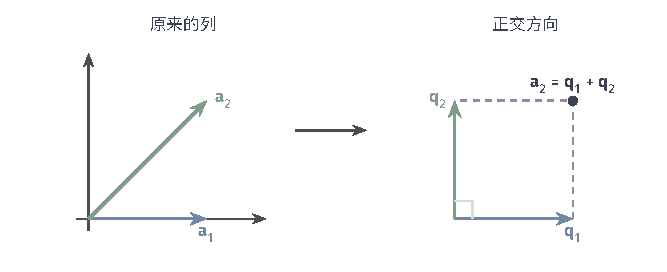
\includegraphics[width=112mm]{figures/00-shared/mathematical-preliminaries-upper/02-linear-spaces/tikz/comprehension-additions/linear-qr-columns.pdf}
  \caption{QR把列的方向和组合系数分开。取$\bm a_1=(1,0)^\top$、$\bm a_2=(1,1)^\top$，
  正交化得到$\bm q_1=(1,0)^\top$、$\bm q_2=(0,1)^\top$，并有$\bm a_1=\bm q_1$、
  $\bm a_2=\bm q_1+\bm q_2$，故$\bm R=\left[\begin{smallmatrix}1&1\\0&1\end{smallmatrix}\right]$。
  虚线补出第二列的分量。}
  \label{fig:vol1-add-linear-qr-columns}
\end{figure}

这一分解的用处在于，涉及列空间的计算可以改在标准正交的$\bm Q$上进行，坐标由内积直接读出，不必再解Gram方程；第~\ref{chap:linear-equations-and-optimization}章解方程与最小二乘问题时正是这样使用它的。

\subsubsection{列相关时的处理}

定理~\ref{thm:ls-gram-schmidt}要求各列线性无关。若不满足，某一步会出现$\bm u_j=\bm0$：由正交分解，这恰好说明$\bm a_j$已在前面方向张成的空间中，没有带来新方向。这时不能对零向量归一化，应跳过这一列，只在$\bm R$中记下它的系数$\langle\bm a_j,\bm q_i\rangle$；跳过它不影响后续各列，因为张成的空间没有变。

全部处理完以后，留下的$\bm q$个数等于列空间的维数$r=\operatorname{rank}\bm A$，仍有$\bm A=\bm Q\bm R$，其中$\bm Q\in\mathbb R^{m\times r}$的列是列空间的标准正交基，$\bm R\in\mathbb R^{r\times d}$的各行从左到右第一个非零元的位置逐行右移；$r<d$时$\bm R$不是方阵，不能求逆。下面是最小的例子。
\begin{example}[列相关时跳过零余量]
\label{ex:ls-qr-dependent-columns}
给定：$\bm A=[\bm a_1\ \bm a_2]$，$\bm a_1=(1,0)^\top$、$\bm a_2=(2,0)^\top$。

计算：$\bm q_1=\bm a_1$。$\langle\bm a_2,\bm q_1\rangle=2$，扣除后$\bm u_2=\bm a_2-2\bm q_1=\bm0$，所以跳过$\bm a_2$，只在$\bm R$中记下系数$2$。于是$r=1$，
\[
\begin{gathered}
\bm Q=\begin{bmatrix}1\\0\end{bmatrix}\\
\bm R=\begin{bmatrix}1&2\end{bmatrix}\\
\bm Q\bm R=\begin{bmatrix}1&2\\0&0\end{bmatrix}=\bm A .
\end{gathered}
\]

结论：列空间仍是$x$轴，$\bm Q$的一列构成它的标准正交基，$\operatorname{rank}\bm A=1$。
\end{example}
于是在精确算术下，同一过程也给出列空间的一组标准正交基与矩阵的秩。有限精度下扣除后的余量很少恰好为零，怎样判断它“算作零”、怎样改写扣除顺序以减少正交性的损失，属于数值计算问题，在第~\ref{sec:ls-numerical-sensitivity}节讨论。

\subsection{正交投影}

标准正交基使子空间的分量可以逐一读出。把这些分量合在一起，就得到离原向量最近的子空间向量。

\paragraph{向子空间的正交分解}
若$\bm q_1,\ldots,\bm q_r$是子空间$U$的标准正交基，第~\ref{sec:ls-orthogonality}节正交直和中的Gram方程变成$\bm a=(\langle\bm q_i,\bm x\rangle)_i$，分解直接写出：
\begin{equation}
 \bm x=\underbrace{\sum_{j=1}^r\langle\bm x,\bm q_j\rangle\bm q_j}_{\bm u\in U}+\underbrace{\Bigl(\bm x-\sum_{j=1}^r\langle\bm x,\bm q_j\rangle\bm q_j\Bigr)}_{\bm r\in U^\perp}.
 \label{eq:ls-orthonormal-projection}
\end{equation}
$\bm u$称为$\bm x$在$U$上的正交投影。$\bm u$与$\bm r$正交，由勾股定理$\lVert\bm x\rVert^2=\lVert\bm u\rVert^2+\lVert\bm r\rVert^2\geq\sum_{j=1}^r\langle\bm x,\bm q_j\rangle^2$：沿一部分标准正交方向读出的系数平方和不超过总长度的平方，等号恰在$\bm x\in U$时成立。对任意$\bm v\in U$，$\bm x-\bm v=(\bm x-\bm u)+(\bm u-\bm v)$的两项分别属于$U^\perp$和$U$。由勾股定理，
\[
 \lVert\bm x-\bm v\rVert^2=\lVert\bm x-\bm u\rVert^2+\lVert\bm u-\bm v\rVert^2\geq\lVert\bm x-\bm u\rVert^2.
\]
等号只在$\bm v=\bm u$时成立，所以$\bm u$是唯一的最近点。一般范数下的最近点可能不唯一；这里的唯一性来自内积所确定的正交分解。

在欧氏坐标下，把$\bm q_1,\ldots,\bm q_r$排成矩阵$\bm Q$，投影写成$P\bm x=\bm Q\bm Q^\top\bm x$。由于$\bm Q^\top\bm Q=\bm I$，投影矩阵$\bm P=\bm Q\bm Q^\top$满足$\bm P^2=\bm P$与$\bm P^\top=\bm P$：投影一次后再投影不再改变结果，配对中也可以把投影移到另一侧。$\bm Q$不是方阵时，$\bm P$通常不是整个空间的单位矩阵，它只保留$U$中的分量。非正交基同样可以通过前面得到的Gram方程计算投影；实际求解时不必显式形成逆矩阵。

\begin{example}[用标准正交基重算正交分解]
\label{ex:ls-orthonormal-projection-line}
给定：$U=\operatorname{span}\{\bm q_1\}$，$\bm q_1=(1,1,1)^\top/\sqrt3$，$\bm y=(1,1.1,0.9)^\top$。

计算：$\langle\bm y,\bm q_1\rangle=3/\sqrt3=\sqrt3$，投影为$\sqrt3\,\bm q_1=(1,1,1)^\top$，余量为$(0,0.1,-0.1)^\top$，它与$\bm q_1$正交。

结论：结果与示例~\ref{ex:ls-orthogonal-decomposition-line}相同，但这里不需要解Gram方程。
\end{example}
标准正交基让投影系数可以逐个读出，接下来把这一投影看作线性映射。

\paragraph{投影矩阵}
\label{sec:ls-projection-matrices}

求出的最近点随目标线性变化：$\bm y_1,\bm y_2$的正交分解相加、数乘后仍是正交分解，由分解的唯一性，
最近点也随之相加、数乘。所以$\bm y\mapsto\bm p$是一个线性映射，称为到$U$的正交投影。
本部分把它写成矩阵，并回答：拿到一个矩阵，怎样判断它是不是正交投影。

\paragraph{正交投影、斜投影与幂等}

设$\bm Q$的列是$U$的标准正交基。由$\bm p=\sum_j\langle\bm q_j,\bm y\rangle\bm q_j=\bm Q\bm Q^\top\bm y$，
标准内积下到$U$的正交投影是
\begin{equation}
\begin{gathered}
\bm P_U=\bm Q\bm Q^\top\\
\bm P_U^\top=\bm P_U\\
\bm P_U^2=\bm P_U.
\end{gathered}
\label{eq:linear-algebra-orthogonal-projector}
\end{equation}
两条性质都可以直接验证。由$\bm Q^\top\bm Q=\bm I$，$\bm P_U^2=\bm Q(\bm Q^\top\bm Q)\bm Q^\top=\bm Q\bm Q^\top$，
即幂等：已经在$U$中的点再投影一次不变。$(\bm Q\bm Q^\top)^\top=\bm Q\bm Q^\top$，即对称。
此外$\operatorname{range}\bm P_U=\operatorname{range}\bm Q=U$。

幂等性只说明这是某种投影，并不说明是最近点映射。一般的幂等矩阵$\bm P$把$\bm y$分成$\bm P\bm y$与
$\bm y-\bm P\bm y$两部分，前者在像中，后者在零空间中（因为$\bm P(\bm y-\bm P\bm y)=\bm P\bm y-\bm P^2\bm y=\bm0$），
但两部分不必正交。这种映射称为\term{斜投影}（oblique projection）。

\begin{example}[反例：幂等而不对称的投影]
\label{ex:ls-oblique-projection}
取$\bm P=\left[\begin{smallmatrix}1&-1\\0&0\end{smallmatrix}\right]$。直接相乘得$\bm P^2=\bm P$，所以它幂等；
它把$(y_1,y_2)^\top$送到$x$轴上的$(y_1-y_2,0)^\top$。残差$\bm y-\bm P\bm y=(y_2,y_2)^\top$与$x$轴方向$(1,0)^\top$的内积是$y_2$，
$y_2\neq0$时不为零，所以$\bm P\bm y$不是$x$轴上离$\bm y$最近的点。这个$\bm P$也不对称：$\bm P^\top\neq\bm P$。
\end{example}

对称性正是正交的条件：若$\bm P$幂等且对称，对任意$\bm y,\bm z$有
$(\bm y-\bm P\bm y)^\top\bm P\bm z=\bm y^\top(\bm P-\bm P^\top\bm P)\bm z=\bm y^\top(\bm P-\bm P^2)\bm z=0$，
残差与整个像正交，由正交性判据，$\bm P$就是到其像的正交投影。
所以判别分两步：先验幂等，判断是不是投影；再验对称，判断是不是正交投影。

\section{线性泛函的内积表示与伴随}
\label{sec:ls-adjoints}

第~\ref{sec:ls-dual-spaces}节的读取规则属于对偶空间，与被读取的向量不在同一个空间；转置在那里是对偶映射的矩阵。有了内积，读取可以写成与一个固定向量的配对，对偶映射也就变成内积空间之间的映射，称为伴随。第~\ref{sec:ls-orthogonality}节证明四个基本子空间的正交关系时，用到的正是它在欧氏内积下的形式：作用在左侧向量上的$\bm A$可以改写成作用在右侧向量上的$\bm A^\top$。第~\ref{chap:linear-analysis}章的对称矩阵与谱分解、第~\ref{chap:linear-equations-and-optimization}章的加权最小二乘，都要用到这种搬动。

\subsection{线性泛函的内积表示}
\phantomsection
\label{sec:ls-riesz-representation}
在$\mathbb R^d$的欧氏内积下，加权读取$\varphi(\bm x)=\bm a^\top\bm x$就是与向量$\bm a$的内积。一般有限维内积空间中，每个读取也都能这样写。
\begin{theorem}[有限维Riesz表示定理]
\label{thm:ls-riesz-representation}
设$V$是有限维内积空间。对每个$\varphi\in V^*$，存在唯一的$\bm v_\varphi\in V$，使$\varphi(\bm x)=\langle\bm x,\bm v_\varphi\rangle$对所有$\bm x\in V$成立。
\end{theorem}
\begin{proof}
取$V$的一组标准正交基$\bm q_1,\ldots,\bm q_d$（第~\ref{sec:ls-orthonormal-basis-construction}节），令$\bm v_\varphi=\sum_j\varphi(\bm q_j)\bm q_j$。由式~\eqref{eq:ls-orthonormal-expansion}，$\bm x=\sum_j\langle\bm x,\bm q_j\rangle\bm q_j$，于是
\[
 \varphi(\bm x)=\sum_j\langle\bm x,\bm q_j\rangle\varphi(\bm q_j)=\Bigl\langle\bm x,\sum_j\varphi(\bm q_j)\bm q_j\Bigr\rangle=\langle\bm x,\bm v_\varphi\rangle.
\]
若$\bm v,\bm v'$都满足要求，则$\langle\bm x,\bm v-\bm v'\rangle=0$对一切$\bm x$成立，取$\bm x=\bm v-\bm v'$得$\bm v=\bm v'$。
\end{proof}
对应$\varphi\mapsto\bm v_\varphi$保持线性组合（由表示向量的唯一性），并且每个$\bm v$都表示读取$\langle\cdot,\bm v\rangle$，所以它是$V^*$到$V$的双射。在它之下，标准正交基的对偶基就是这组基本身，因为第$j$个坐标读取是$\bm x\mapsto\langle\bm x,\bm q_j\rangle$。对一般的基，对偶基对应的向量与原基不同：图~\ref{fig:ls-dual-basis-readout}中的红色箭头$\bm b^1,\bm b^2$正是对偶读取$\varphi_1,\varphi_2$在欧氏内积下对应的向量。

表示向量依赖内积，读取本身却不依赖。在$\mathbb R^d$上取加权内积$\langle\bm x,\bm y\rangle_{\bm M}=\bm x^\top\bm M\bm y$，同一个读取$\varphi(\bm x)=\bm a^\top\bm x=\bm x^\top\bm M(\bm M^{-1}\bm a)$对应的向量是$\bm M^{-1}\bm a$，而不是$\bm a$。函数空间中也是如此。
\begin{example}[积分读取在两点内积下的表示向量]
\label{ex:ls-riesz-integral-two-point}
给定：$P_1$上的内积$\langle f,g\rangle=f(0)g(0)+f(1)g(1)$与读取$\varphi(f)=\int_0^1f(t)\,\mathrm dt$。

计算：对$f=a+bt$，$\varphi(f)=a+b/2$。另一方面，$f$与常数函数$\tfrac12$的内积为
\[
 \Bigl\langle f,\tfrac12\Bigr\rangle=\tfrac12\bigl(f(0)+f(1)\bigr)=\tfrac12(a+a+b)=a+\frac b2 .
\]

结论：$\bm v_\varphi$是常数函数$\tfrac12$。这也说明梯形公式$\tfrac12\bigl(f(0)+f(1)\bigr)$对一次函数精确。
\end{example}
表示向量还给出读取的大小。由Cauchy--Schwarz不等式，$|\varphi(\bm x)|\leq\lVert\bm x\rVert\,\lVert\bm v_\varphi\rVert$；$\bm v_\varphi\neq\bm0$时取$\bm x=\bm v_\varphi/\lVert\bm v_\varphi\rVert$可取到等号，所以第~\ref{sec:ls-finite-dimensional-sequences}节定义的$\lVert\varphi\rVert_*$等于$\lVert\bm v_\varphi\rVert$。

\subsection{伴随与特殊线性算子}
对偶映射把输出端的读取$f$传回输入端，得到读取$f\circ T$。若把读取都换成表示它的向量，就得到下面的定义。

设$T:V\to W$是两个有限维实内积空间之间的线性映射。若存在$T^\star:W\to V$使
\begin{equation}
 \langle T\bm x,\bm y\rangle_W=\langle\bm x,T^\star\bm y\rangle_V
 \label{eq:ls-adjoint-pairing}
\end{equation}
对所有$\bm x\in V$、$\bm y\in W$成立，则$T^\star$称为$T$的\term{伴随}（adjoint）。
\label{def:linear-algebra-adjoint}

伴随总存在且唯一。固定$\bm y\in W$，$\bm x\mapsto\langle T\bm x,\bm y\rangle_W$是$V$上的线性泛函，由定理~\ref{thm:ls-riesz-representation}，存在唯一的向量使它写成与该向量的内积，把这个向量记为$T^\star\bm y$。$T^\star$对$\bm y$线性：$\langle\bm x,aT^\star\bm y+bT^\star\bm y'\rangle_V=a\langle T\bm x,\bm y\rangle_W+b\langle T\bm x,\bm y'\rangle_W=\langle T\bm x,a\bm y+b\bm y'\rangle_W$，由表示向量的唯一性，$T^\star(a\bm y+b\bm y')=aT^\star\bm y+bT^\star\bm y'$。

用对偶映射的语言说，若把$\bm y\in W$看成读取$\langle\cdot,\bm y\rangle_W$，则$T'$把它送到读取$\langle T\,\cdot,\bm y\rangle_W=\langle\cdot,T^\star\bm y\rangle_V$：伴随就是借内积把读取换成向量以后的对偶映射。

具体计算时取$V,W$的基。由坐标下的内积公式，两边的内积写成$\langle\bm x,\bm x'\rangle_V=\bm x^\top\bm M_V\bm x'$、$\langle\bm y,\bm y'\rangle_W=\bm y^\top\bm M_W\bm y'$（这里$\bm x,\bm y$等指坐标），其中$\bm M_V,\bm M_W$是两组基的Gram矩阵，对称正定因而可逆；设$T$的矩阵为$\bm A$，伴随的矩阵为$\bm B$。式~\eqref{eq:ls-adjoint-pairing}要求$(\bm A\bm x)^\top\bm M_W\bm y=\bm x^\top\bm M_V\bm B\bm y$对所有$\bm x,\bm y$成立；取$\bm x,\bm y$为标准坐标向量逐个比较元素，这等价于$\bm A^\top\bm M_W=\bm M_V\bm B$，即
\begin{equation}
 \bm B=\bm M_V^{-1}\bm A^\top\bm M_W.
 \label{eq:ls-weighted-adjoint}
\end{equation}
两端都取标准正交基时，$\bm M_V,\bm M_W$都是单位矩阵，伴随矩阵就是$\bm A^\top$，与对偶映射的矩阵相同；两边权重不同时，伴随既不是单纯转置，也不是转置再求逆。下面的例子说明这一点。
\begin{example}[加权内积下的伴随]
\label{ex:ls-weighted-adjoint}
给定：$V=W=\mathbb R^2$都取加权内积$\langle\bm x,\bm y\rangle_{\bm M}=\bm x^\top\bm M\bm y$，$\bm M=\operatorname{diag}(4,1)$；$T\bm x=\bm A\bm x$，$\bm A=\left[\begin{smallmatrix}0&1\\0&0\end{smallmatrix}\right]$。

计算：由式~\eqref{eq:ls-weighted-adjoint}，
\[
 \bm B=\bm M^{-1}\bm A^\top\bm M
 =\begin{bmatrix}1/4&0\\0&1\end{bmatrix}\begin{bmatrix}0&0\\1&0\end{bmatrix}\begin{bmatrix}4&0\\0&1\end{bmatrix}
 =\begin{bmatrix}0&0\\4&0\end{bmatrix}.
\]
直接核对：$\bm A\bm x=(x_2,0)^\top$，$\langle\bm A\bm x,\bm y\rangle_{\bm M}=4x_2y_1$；$\bm B\bm y=(0,4y_1)^\top$，$\langle\bm x,\bm B\bm y\rangle_{\bm M}=x_2\cdot4y_1$，两者相等。

结论：伴随矩阵是$\left[\begin{smallmatrix}0&0\\4&0\end{smallmatrix}\right]$，而不是$\bm A^\top=\left[\begin{smallmatrix}0&0\\1&0\end{smallmatrix}\right]$。
\end{example}
对偶映射的矩阵总是$\bm A^\top$，差别来自读取与向量之间的对应$\bm a\mapsto\bm M^{-1}\bm a$随内积改变。四个基本子空间正交关系的证明只用到配对恒等式，所以对一般内积空间同样有$\ker T^\star=(\operatorname{im}T)^\perp$、$\ker T=(\operatorname{im}T^\star)^\perp$。

\paragraph{伴随的运算规则}
伴随与组合的规则由配对定义逐项推出：
\[
 \begin{gathered}
(T+S)^\star=T^\star+S^\star\\
(cT)^\star=c\,T^\star\\
(TS)^\star=S^\star T^\star\\
T^{\star\star}=T.
 \end{gathered}
\]
例如$\langle TS\bm x,\bm y\rangle=\langle S\bm x,T^\star\bm y\rangle=\langle\bm x,S^\star T^\star\bm y\rangle$，复合伴随的次序与乘积转置一样反转；恒等映射的伴随是自身。图~\ref{fig:ls-adjoint-action-transfer}把这种配对方向的搬回画成示意图。

伴随也不是逆：逆把输出复原成输入，伴随只把读取方向换一侧。
\begin{example}[反例：伴随不是逆]
\label{ex:ls-adjoint-not-inverse}
给定：非零内积空间$V$上的算子$T=2\operatorname{id}$。

验证：$\langle2\bm x,\bm y\rangle=\langle\bm x,2\bm y\rangle$对一切$\bm x,\bm y$成立，所以$T^\star=2\operatorname{id}$；而$T^{-1}=\tfrac12\operatorname{id}$。

结论：$T^\star\neq T^{-1}$。
\end{example}
\begin{figure}[!htb]
  \centering
  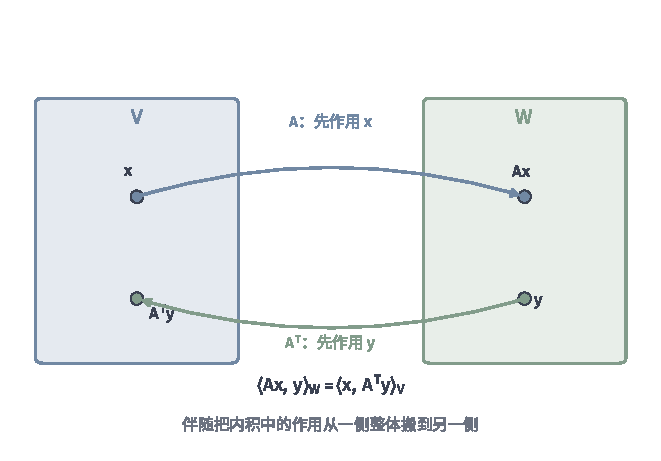
\includegraphics[width=112mm]{figures/00-shared/mathematical-preliminaries-upper/02-linear-spaces/matplotlib/ls-adjoint-action-transfer/ls-adjoint-action-transfer.pdf}
  \caption{内积伴随把输出端的配对搬回输入端。左：$T:V\to W$把$\bm x$映成$T\bm x$，与$\bm y\in W$配对；右：伴随$T^\star:W\to V$把$\bm y$映回$T^\star\bm y\in V$，使$\langle T\bm x,\bm y\rangle_W=\langle\bm x,T^\star\bm y\rangle_V$。标准欧氏内积下$T^\star$就是转置，是配对方向的反转而非逆作用。箭头与空间为解析示意。}
  \label{fig:ls-adjoint-action-transfer}
\end{figure}

\paragraph{自伴、正交与正规算子}
对算子$T:V\to V$，伴随仍是$V$上的算子，可以与$T$比较。若$T^\star=T$，称$T$为\term{自伴}（self-adjoint）算子，标准坐标下对应对称矩阵。若$Q^\star Q=\operatorname{id}$，则$Q$保持内积：$\langle Q\bm x,Q\bm y\rangle=\langle\bm x,Q^\star Q\bm y\rangle=\langle\bm x,\bm y\rangle$，称为正交算子；标准坐标下它对应第~\ref{sec:ls-orthogonal-matrices}节的正交矩阵，且由方阵的单侧逆即双侧逆，$Q^{-1}=Q^\star$。满足$TT^\star=T^\star T$的算子称为\term{正规}（normal）算子，自伴与正交都属于它。这些类别的谱性质在第~\ref{chap:linear-analysis}章展开，这里只给出定义。

\paragraph{复空间中的泛函表示与伴随}
复空间沿用前述“第一变量共轭线性、第二变量线性”的约定。线性泛函应写成$\varphi(\bm x)=\langle\bm v,\bm x\rangle$：$\bm x$处于线性槽位。若$\bm q_1,\ldots,\bm q_d$是标准正交基，则$\bm v=\sum_j\overline{\varphi(\bm q_j)}\bm q_j$；直接代入各基向量可核对其读数。表示向量随泛函作共轭线性变化，与实空间中的线性对应不同。

例如在$\mathbb C$的标准内积$\langle v,z\rangle=\overline v z$下，泛函$\varphi(z)=(1+\mathrm i)z$对应$ v=1-\mathrm i$。代入便有$\overline v z=(1+\mathrm i)z$；若把两个槽位交换，就会得到关于$z$共轭线性的表达式。这个一维核验说明，共轭来自内积约定，不能从实数公式中直接删去。

两个复内积空间之间的伴随满足$\langle T\bm x,\bm y\rangle_W=\langle\bm x,T^\star\bm y\rangle_V$。在标准正交基下，$T$的矩阵若为$\bm A$，伴随的矩阵就是$\bm A^*$；若两端基的Gram矩阵为$\bm M_V,\bm M_W$，则为$\bm M_V^{-1}\bm A^*\bm M_W$。这与代数对偶映射的矩阵$\bm A^\top$不同：后者只复合线性泛函，不涉及内积和共轭。复空间中自伴矩阵满足$\bm A=\bm A^*$，保内积的方阵满足$\bm A^*\bm A=\bm I$，称为酉矩阵。

\section{本章小结}
\label{sec:ls-normed-inner-product-summary}

范数给向量规定大小，从而可以比较误差并定义收敛。有限维空间中的范数彼此等价，向量列收敛等价于逐坐标收敛；这些空间及其子空间都是完备的。对偶范数把输入大小的限制转化为线性泛函的最大读数，商范数则衡量忽略一个子空间中的差别以后剩余的大小。

内积进一步给出角度和正交。Gram矩阵记录一组向量的两两内积，正交分解把向量拆成子空间内的部分与垂直部分；正交投影是内积诱导距离下唯一的最近点。标准正交基简化配对与坐标计算，线性泛函的内积表示和伴随则连接了上一章的代数对偶与本章的几何结构。

这些结论为下一章寻找线性作用的简单表示提供了工具。有限维中的闭性、完备性和连续性不能不加条件地推广到无限维空间。

